\documentclass{beamer}

\usepackage[utf8]{inputenc}
\usepackage{default}

\mode<presentation>
%{ \usetheme{boxes} }


\usetheme{Madrid}

\usepackage{times}
\usepackage{graphicx}
\usepackage{tabulary}
\usepackage{listings}
\usepackage{verbatimbox}
\usepackage{graphicx}
\usepackage{lmodern}
\usepackage[absolute,overlay]{textpos}
\usepackage{pgfpages}
\usepackage{color}

\usepackage{multicol}

\definecolor{mycolorcli}{RGB}{53,154,26}
\definecolor{mycolorcode}{RGB}{0,0,255}
\definecolor{mycolordef}{RGB}{255,0,0}

\pgfdeclareimage[height=1.0cm]{logo_rcc}{graphs/logo_rcc.png}
\setlength{\TPHorizModule}{1mm}
\setlength{\TPVertModule}{1mm}
\newcommand{\RCCLogo}{
\begin{textblock}{14}(1.5,1.5)
  \pgfuseimage{logo_rcc}
\end{textblock}
}


\title{\huge{Distributed Programming with MPI in C}}
\author{Igor Yakushin \\ \texttt{ivy2@uchicago.edu}}
%\date{September 10, 2017}

\definecolor{ChicagoMaroon}{RGB}{128,0,0}

\setbeamercolor{title}{bg=ChicagoMaroon}

\begin{document}

\setbeamertemplate{navigation symbols}{}

\setbeamercolor{fcolor}{fg=white,bg=ChicagoMaroon}
\setbeamertemplate{footline}{
\begin{beamercolorbox}[ht=4ex,leftskip=1.4cm,rightskip=.3cm]{fcolor}
\hrule
\vspace{0.1cm}
   \hfill \insertshortdate \hfill \insertframenumber/\inserttotalframenumber
\end{beamercolorbox}
}

\setbeamercolor{frametitle}{bg=ChicagoMaroon,fg=white}

\begin{frame}
\RCCLogo
\titlepage
\end{frame}

\section{Introduction}
\begin{frame}[fragile]
  \frametitle{Introduction}

\begin{itemize}
\item {\color{mycolordef}\textbf{M}}essage {\color{mycolordef}\textbf{P}}assing {\color{mycolordef}\textbf{I}}nterface
\item Standard for distributed computing implemented as a library
\item MPI-1 (1994)
\item Current standard: MPI-3.1 (2015)
\item About 250 routines
\item Available for C (native), Fortran, Python (mpi4py), ...
\item Some popular implementations:
  \begin{itemize}
    \item mpich
    \item mvapich
    \item Intel MPI - we use in this tutorial
    \item openmpi
  \end{itemize}
\item MPI runs the same program on different nodes/cores. Each process is assigned a  {\color{mycolordef}\textbf{rank}}. 
  Using \textcolor{blue}{if} statement, a program can do different things for different ranks, exchange messages between different ranks
\item In general (with one exception), there is no shared memory like in multithreading.
\end{itemize}

\end{frame}

\section{When to use MPI?}
\begin{frame}[fragile]
  \frametitle{When to use MPI?}
  \begin{itemize}
    \item Use MPI when your program requires more computing power or more memory than a single node can provide and different parts of the program need to exchange data. For example:
      \begin{itemize}
        \item Solving PDE on a big grid: 
          \begin{itemize}
          \item divide the grid into patches and distribute the patches across MPI ranks
          \item make one time step on each patch independently
          \item exchange boundaries via MPI messages
          \end{itemize}
        \item Working with matrixes that do not fit in memory of a single node
      \end{itemize}
    \item You do not need MPI to run embarassingly parallel computations that can run on different nodes without exchanging data. For example:
      \begin{itemize}
      \item Simulations that use different set of parameters can run independently on different nodes
      \item Data analysis pipeline parallelized over data
      \end{itemize}
  \end{itemize}
\end{frame}


\section{Where MPI can be used?}
\begin{frame}[fragile]
  \frametitle{Where MPI can be used?}
  \begin{itemize}
  \item One can use MPI on a single host running on local cores (useful for learning)
{\color{mycolorcli}
\begin{verbatim}
  mpirun -np 2 <yourprogram>
\end{verbatim}
}
  \item One can use MPI on a cluster without a scheduler provided that a user can 
    ssh from any host to any host without password (using ssh key with empty passphrase)
{\color{mycolorcli}
\begin{verbatim}
  mpirun -np 2 -hostfile <file with a list of hosts> 
                         <yourprogram>
\end{verbatim}
}
\item One can use MPI on a cluster with a scheduler, for example Slurm. 
  In that case one prepares a batch script requesting resources (number of nodes, cores per node, 
  memory, time, etc.) and
  specifies the command to run:
{\color{mycolorcli}
\begin{verbatim}
  mpirun <yourprogram>
\end{verbatim}
}
The scheduler takes care of distributing the computation among the nodes/cores given to the application
\end{itemize}
\end{frame}


\section{How to login to midway 2}
\begin{frame}[fragile]
  \frametitle{How to login to midway 2}
  \begin{itemize}
  \item {\color{mycolorcli}\verb|ssh -Y <userid>@midway2.rcc.uchicago.edu|} or use ThinLinc: 
    {\color{mycolorcli}\verb|https://midway2.rcc.uchicago.edu|}.
  \item If you do not have an account on midway, use yubikeys:
 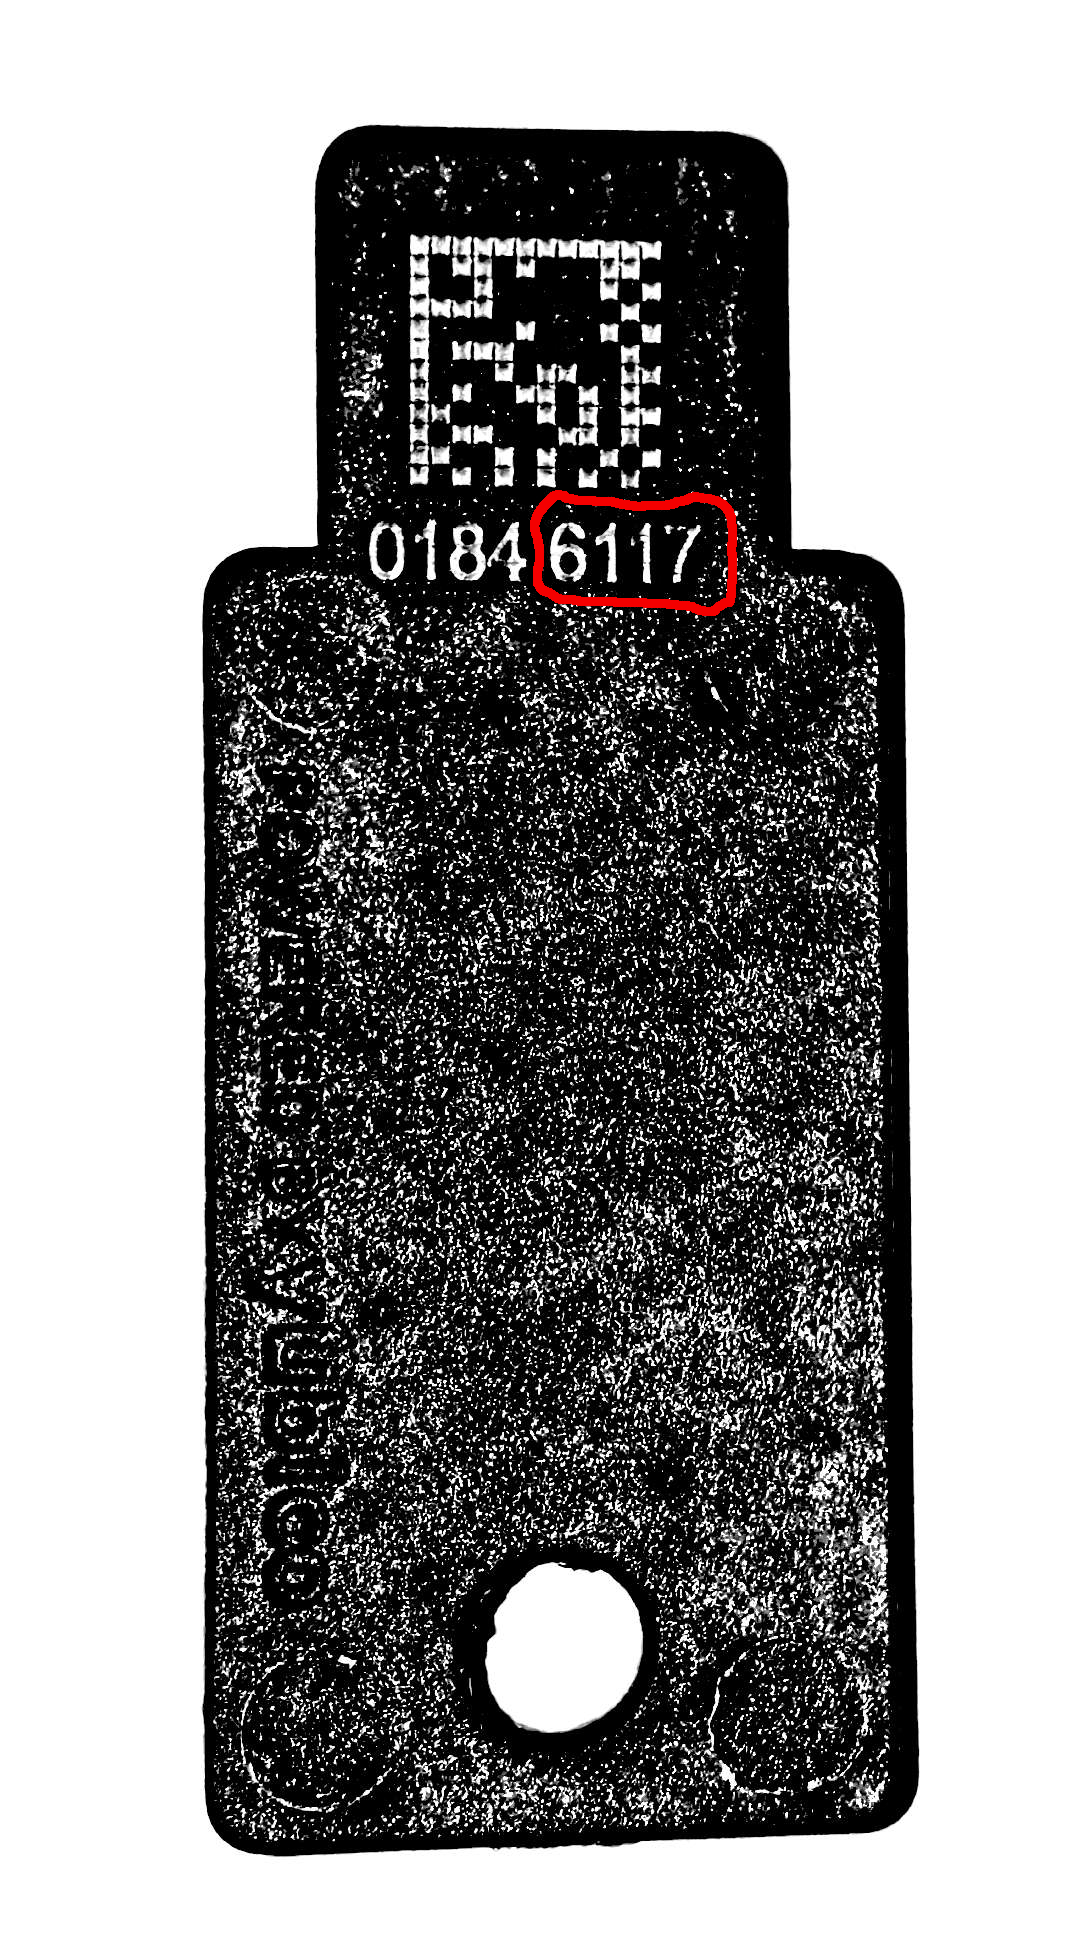
\includegraphics[width=2.3cm]{icons/yubikey1a.jpg}
 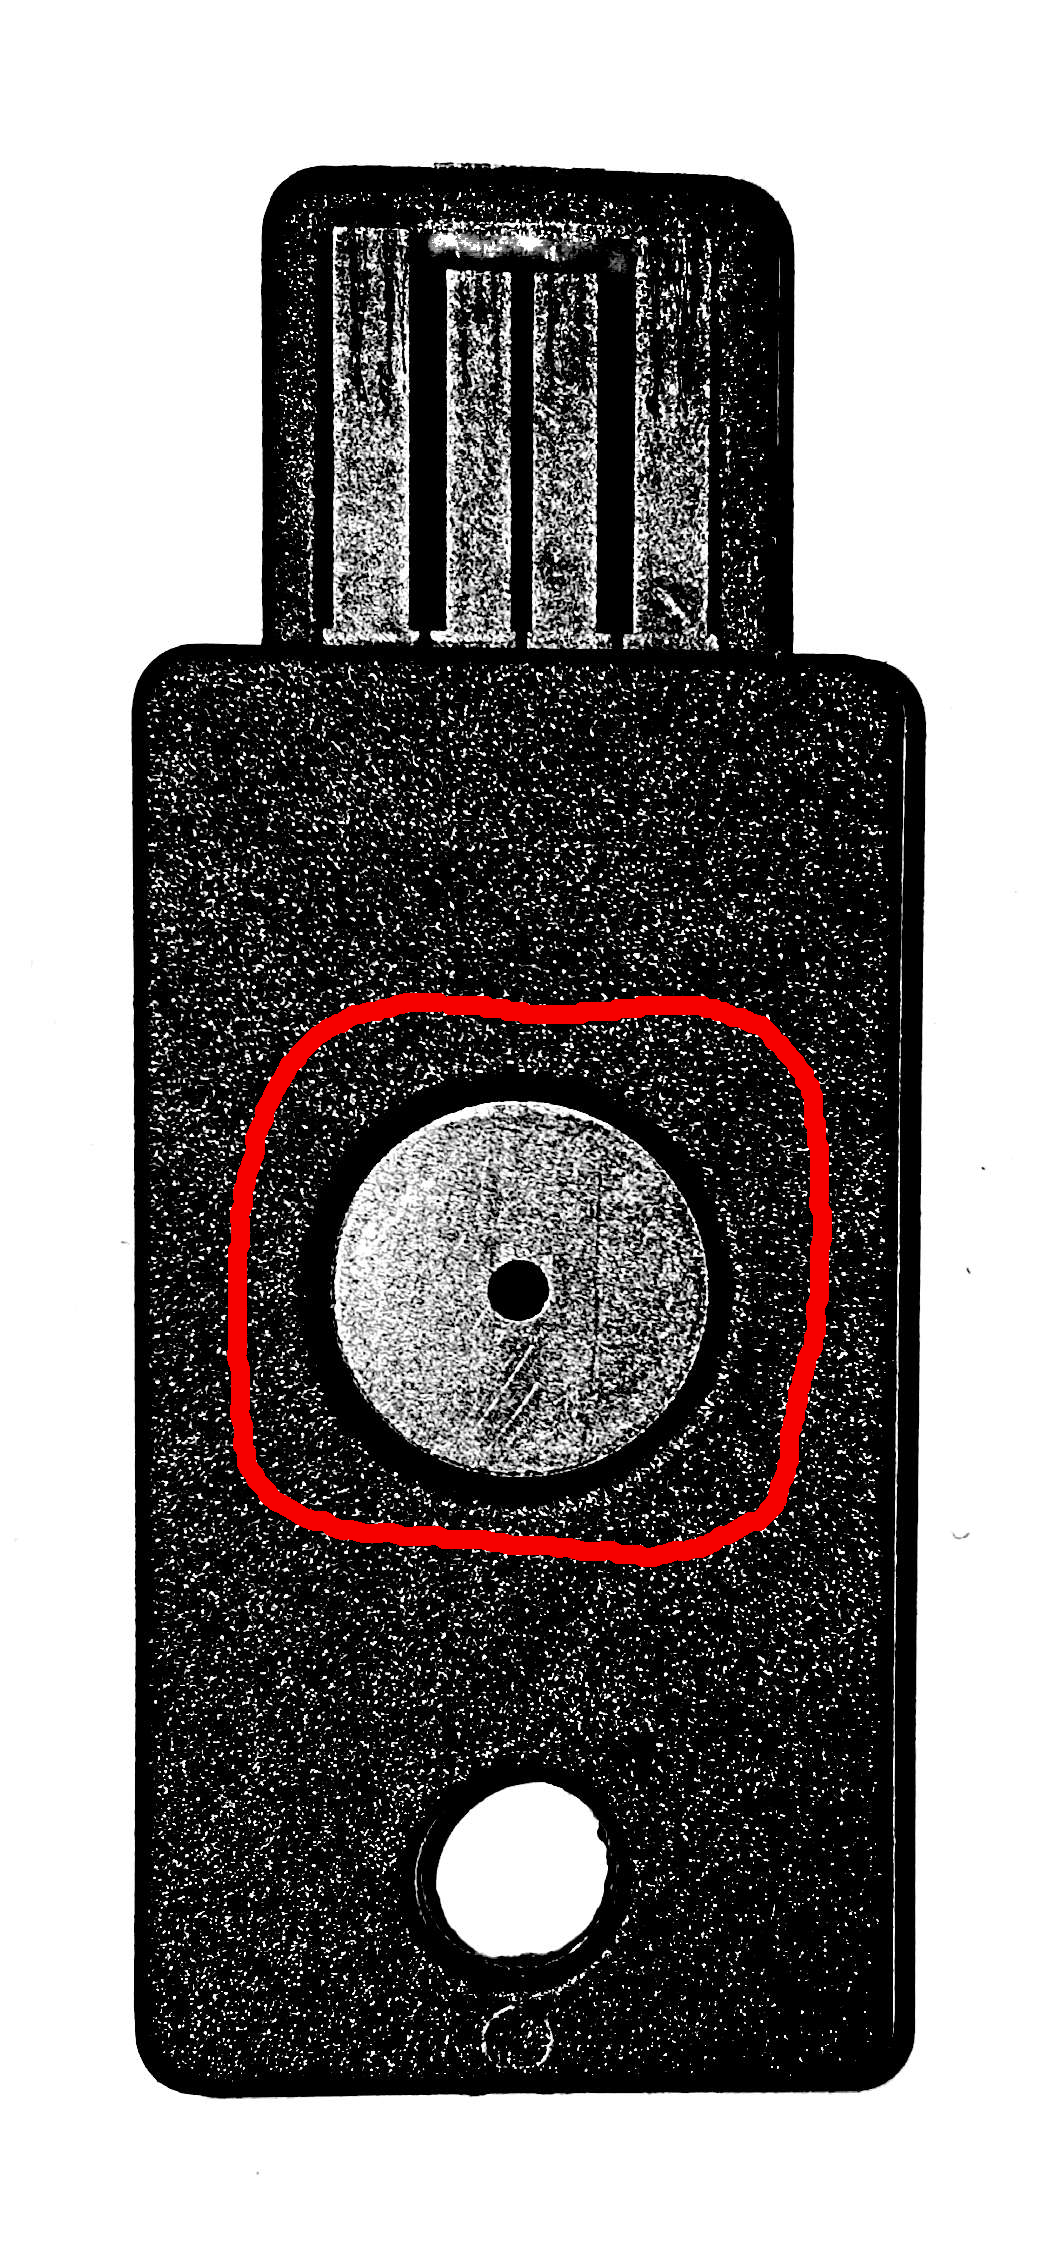
\includegraphics[width=2cm]{icons/yubikey2a.jpg}
 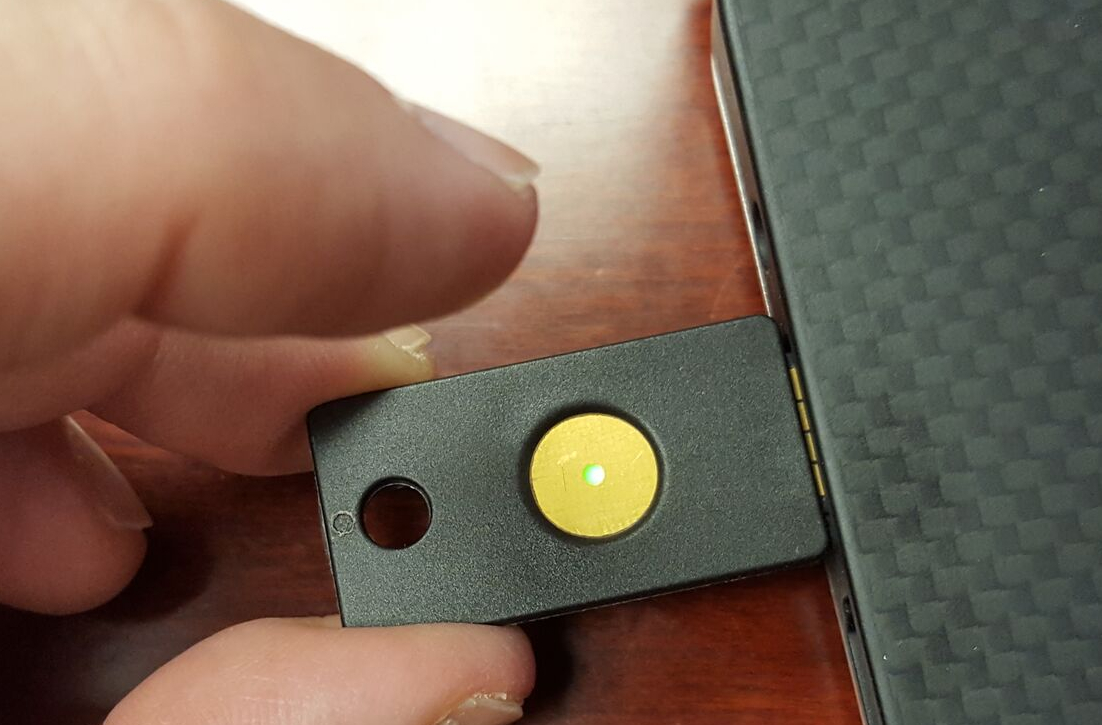
\includegraphics[width=5cm]{icons/yubikey3a.jpg}
 \item Use last 4 digits of yubikey {\color{mycolorcli}\verb|<XXXX>|} as part of userid:
{\color{mycolorcli}
\begin{verbatim}
ssh -Y rccguest<XXXX>@midway2.rcc.uchicago.edu
\end{verbatim}
}
Push the button when asked for password
{\tiny
{\color{mycolorcli}
\begin{verbatim}
git clone https://git.rcc.uchicago.edu/ivy2/MPI_Introduction_C.git
cd MPI_Introduction_C/labs; source env.sh; cd 1
\end{verbatim}
}
}
\end{itemize}
\end{frame}


\section{Simplest MPI program: Lab1}
\subsection{C/C++}
\begin{frame}[fragile]
  \frametitle{Simplest MPI program: Lab1: C/C++}
{\color{mycolorcode}
{\small
\begin{verbatim}
#include <stdio.h>
#include "mpi.h"
int main(int argc, char **argv)
{
  int size, rank;
  char host[1024];
  int hostlen;
  MPI_Init(&argc,&argv);
  MPI_Comm_size(MPI_COMM_WORLD, &size);
  MPI_Comm_rank(MPI_COMM_WORLD, &rank);
  MPI_Get_processor_name(host, &hostlen);
  printf("size=%d, rank=%d hostname=%s\n", 
          size, rank, host);
  MPI_Finalize();
}
\end{verbatim}
}
}
\end{frame}

\begin{frame}[fragile]
  \frametitle{Simplest MPI program: Lab1: C/C++}
\begin{itemize}
\item An MPI header is included
\item MPI is initialized at the beginning and finalized at the end
\item We use \textcolor{mycolordef}{Intel MPI} implementation of MPI that comes with Intel Parallel Studio
\item To build the program, use {\color{mycolorcli}mpicc} instead of {\color{mycolorcli}gcc} or 
  {\color{mycolorcli}mpiicc} instead of {\color{mycolorcli}icc}:
{\color{mycolorcli}
\begin{verbatim}
mpicc -o hello hello.c  // uses gcc
or
mpiicc -o hello hello.c // uses Intel icc
\end{verbatim}
}
\item {\color{mycolorcli} \verb|mpicc|}/{\color{mycolorcli} \verb|mpiicc|} is simply a wrapper around compiler, 
  in this case {\color{mycolorcli} \verb|gcc|}/{\color{mycolorcli} \verb|icc|}, 
  that links all the necessary MPI libraries and provides paths to headers
\item To run a program using 2 processes on login node
{\color{mycolorcli}
\begin{verbatim}
mpirun -n 2 ./hello
\end{verbatim}
}
\item Each MPI process executes the same program
\end{itemize}
\end{frame}

\begin{frame}[fragile]
  \frametitle{Simplest MPI program: Lab1: C/C++}
\begin{itemize}
  \item Only MPI processes that use the same {\color{mycolordef}\textbf{communicator}} can talk to each other. 
    For now we are using {\color{mycolorcode}\verb|MPI_COMM_WORLD|} communicator so that all the processes can talk to each other. In general, you might want to use several
    communicators to restrict communication in the program.
  \item The program queries the communicator to find out how many processes use it ({\color{mycolorcode}\verb|size|}) and what is the rank of the current process. 
    Ranks are counted separately for each communicator from {\color{mycolorcode}0} to {\color{mycolorcode}\verb|size-1|}. We also ask for the hostname.
  \item Each process prints size, rank and hostname:
{\small
{\color{mycolorcli}
\begin{verbatim}
size=2, rank=1 hostname=ivy2-XPS-15
size=2, rank=0 hostname=ivy2-XPS-15
\end{verbatim}
}
}
\item The corresponding C++ program looks identical, as far as MPI is concerned, but is compiled with
{\small
{\color{mycolorcli}
\begin{verbatim}
mpic++ -o hello++ hello.C  // using gcc
or
mpiicpc -o hello++ hello.C // using Intel's icpc
\end{verbatim}
}
}
\end{itemize}
\end{frame}

\subsection{Running on the cluster under Slurm}
\begin{frame}[fragile]
  \frametitle{Simplest MPI program: Lab1: running under Slurm}

\begin{itemize}
\item To run the program in batch under Slurm

{\color{mycolorcli}
\begin{verbatim}
sbatch hello.batch
  Submitted batch job 34723042
\end{verbatim}
}

\item One can use {\color{mycolorcli}\verb|squeue|} to monitor the job

  \begin{itemize}
  \item by userid:
    {\color{mycolorcli}
\begin{verbatim}
squeue -u ivy2
\end{verbatim}
    }
  \item by jobid:
    {\color{mycolorcli}
\begin{verbatim}
squeue -j 34723042
\end{verbatim}
    }
  \end{itemize}
\item To kill the job, use
{\color{mycolorcli}
\begin{verbatim}
scancel 34723042
\end{verbatim}
}
\item While the job is running, one can ssh to the corresponding compute node and, for example, run top to see what's going on
\item In {\color{mycolorcli}\verb|hello.out|}
  {\color{mycolorcli}
\begin{verbatim}
size=2, rank=0 hostname=midway2-0002.rcc.local
size=2, rank=1 hostname=midway2-0003.rcc.local
\end{verbatim}
  }
\end{itemize}
\end{frame}

\section{Point-to-point communication}
\subsection{Blocking send/receive: Lab2}
\begin{frame}[fragile]
  \frametitle{P2P communication: blocking send/receive: Lab2}

\begin{itemize}
\item {\color{mycolorcode}\verb|MPI_Send|} function can be used to send data to another rank:
{\color{mycolorcode}
\begin{verbatim}
  int MPI_Send(const void* buf, int count, 
    MPI_Datatype datatype, int dest, int tag, 
    MPI_Comm comm)
\end{verbatim}
}
where
\begin{itemize}
\item {\color{mycolorcode}buf} - array with data
\item {\color{mycolorcode}count} - number of units of datatype ({\color{mycolorcode}\verb|MPI_INT|}, {\color{mycolorcode}\verb|MPI_FLOAT|}, {\color{mycolorcode}\verb|MPI_DOUBLE|}, etc.)
\item {\color{mycolorcode}dest} - rank of the destination process
\item {\color{mycolorcode}tag} - can be used to distinguish one set of messages from another
\end{itemize}
\end{itemize}
\end{frame}

\begin{frame}[fragile]
  \frametitle{P2P communication: blocking send/receive: Lab2}
\begin{itemize}
\item The receiver process must execute {\color{mycolorcode}\verb|MPI_Receive|} to get the message:
{\color{mycolorcode}
\begin{verbatim}
  int MPI_Recv(void* buf, int count, 
    MPI_Datatype datatype, int source, int tag, 
    MPI_Comm comm, MPI_Status *status)
\end{verbatim}
}
\item The receiver might use wildcards instead of source ({\color{mycolorcode}\verb|MPI_ANY_SOURCE|}) and tag ({\color{mycolorcode}\verb|MPI_ANY_TAG|}).
\item To find out the actual source and tag of the received message, one can use {\color{mycolorcode}\verb|status|} which is a structure with the following fields: {\color{mycolorcode}\verb|MPI_SOURCE|}, {\color{mycolorcode}\verb|MPI_TAG|},
and {\color{mycolorcode}\verb|MPI_ERROR|}. A user must allocate {\color{mycolorcode}\verb|MPI_Status|} variable before using it or use {\color{mycolorcode}\verb|MPI_STATUS_IGNORE|} instead.
\item The status argument can also be used to find out the length of the received message:
{\color{mycolorcode}
\begin{verbatim}
  int MPI_Get_count(const MPI_Status *status, 
    MPI_Datatype datatype, int *count)
\end{verbatim}
}
\end{itemize}
\end{frame}

\begin{frame}[fragile]
  \frametitle{P2P communication: blocking send/receive: Lab2}
\begin{itemize}
\item MPI receive calls specify a receive buffer and its size has to be enough for any data sent.
\item In case you really have no idea how much data is being sent and you don't want to overallocate the receive buffer, you can use a probe call.
\item {\color{mycolorcode}\verb|MPI_Probe|} do not copy data but tell that there is a message and you can use {\color{mycolorcode}\verb|MPI_Get_count|} 
to determine its size, allocate a large enough receive buffer and do a regular receive to have the data copied:
{\color{mycolorcode}
\begin{verbatim}
  if(mytid == receiver) {
    MPI_Status status;
    MPI_Probe(sender,0,comm,&status);
    int count;
    MPI_Get_count(&status, MPI_FLOAT, &count);
    float recv_buffer[count];
    MPI_Recv(recv_buffer, count, MPI_FLOAT, 
             sender, 0, comm, MPI_STATUS_IGNORE);
\end{verbatim}
}
\end{itemize}
\end{frame}


\begin{frame}[fragile]
  \frametitle{P2P communication: blocking send/receive: Lab2}
\begin{itemize}
\item Sometimes it is convenient to use combined send/receive command
\item A good use case is when two patches on the grid need to exchange boundaries
\item Executing a single sendrecv is faster and less error prone then making two calls
\end{itemize}
{\color{mycolorcode}
\begin{verbatim}
  int MPI_Sendrecv(const void *sendbuf, int sendcount, 
    MPI_Datatype sendtype, int dest, int sendtag, 
    void *recvbuf, int recvcount, MPI_Datatype recvtype, 
    int source, int recvtag, MPI_Comm comm, 
    MPI_Status *status)
\end{verbatim}
}
\end{frame}


\begin{frame}[fragile]
  \frametitle{P2P communication: blocking send/receive: Lab2}
\begin{itemize}
\item {\color{mycolorcode}\verb|MPI_Send|} and {\color{mycolorcode}\verb|MPI_Receive|} functions are {\color{mycolordef}\textbf{blocking}}: 
\begin{itemize}
\item sender can procede only after it is safe to overwrite the message: it was copied to some buffer but not necessarily delivered yet
\item receive can procede only after the message is delivered
\end{itemize}
\item There are several problems with that:
\begin{itemize}
\item One needs to be very careful while ordering send/receive to avoid {\color{mycolordef}\textbf{deadlock}}. Consider the situation:
\begin{verbatim}
  Process 0:
    receive from 1
    send to 1
  Process 1:
    receive from 0
    send to 0
\end{verbatim}
Both processes are waiting for each other and get stuck.
\item While waiting for send/receive to complete, neither sender nor receiver can do any useful job
\end{itemize}
\end{itemize}
\end{frame}

\subsection{Non-blocking send/receive: Lab3}
\begin{frame}[fragile]
  \frametitle{P2P communication: non-blocking send/receive: Lab3}
\begin{itemize}
\item Non-blocking send/receive calls solve these two problems:
\begin{itemize}
\item The calls return immediately
\item One can either query later if calls are finished or wait for the end of all or some of such calls at some point in the program
\item This allows to overlap computation and communication
\item One needs to be careful not to overwrite the message storage before it is delivered
\end{itemize}
{\color{mycolorcode}
\begin{verbatim}
  int MPI_Isend(const void* buf, int count, 
    MPI_Datatype datatype, int dest, int tag, 
    MPI_Comm comm, MPI_Request *request)

  int MPI_Irecv(void* buf, int count, 
    MPI_Datatype datatype, int source,
    int tag, MPI_Comm comm, 
    MPI_Request *request)
\end{verbatim}
}
\end{itemize}
\end{frame}

\begin{frame}[fragile]
  \frametitle{P2P communication: non-blocking send/receive: Lab3}
\begin{itemize}
\item {\color{mycolorcode}\verb|request|} is used in {\color{mycolorcode}\verb|MPI_Wait|} and {\color{mycolorcode}\verb|MPI_Test|} to test the completion of non-blocking calls
{\color{mycolorcode}
\begin{verbatim}
  int MPI_Wait(MPI_Request *request, 
    MPI_Status *status)
  int MPI_Test(MPI_Request *request, int *flag, 
    MPI_Status *status)
\end{verbatim}
}
\item A call to {\color{mycolorcode}\verb|MPI_Wait|} returns when the operation identified by request is complete and can be used once
\item A call to {\color{mycolorcode}\verb|MPI_Test|} returns \verb|flag=true| if the operation identified by request is complete and can be used multiple times
\item A request object can be deallocated without waiting for the associated communication
to complete: 
{\color{mycolorcode}
\begin{verbatim}
  int MPI_Request_free(MPI_Request *request)
\end{verbatim}
}
\end{itemize}
\end{frame}

\begin{frame}[fragile]
  \frametitle{P2P communication: non-blocking send/receive: Lab3}
\begin{itemize}
\item {\color{mycolorcode}\verb|MPI_Waitall|} allows you to wait for a number of requests and it does not matter in what sequence they are satisfied:
{\color{mycolorcode}
\begin{verbatim}
  int MPI_Waitall(int count, 
    MPI_Request array_of_requests[],
    MPI_Status array_of_statuses[])
\end{verbatim}
}
\item There is also corresponding {\color{mycolorcode}\verb|MPI_Testall|}
\item Instead of waiting/testing for all the requests in the list, one can wait/test for some to happen:
{\color{mycolorcode}
\begin{verbatim}
  int MPI_Waitsome(int incount, 
    MPI_Request array_of_requests[],
    int *outcount, int array_of_indices[],
    MPI_Status array_of_statuses[])
\end{verbatim}
}
\item Waits until at least one of the operations associated with active handles in the list have
completed. Returns in outcount the number of requests from the list {\color{mycolorcode}\verb|array_of_requests|} that
have completed.
\end{itemize}
\end{frame}

\begin{frame}[fragile]
  \frametitle{P2P communication: non-blocking send/receive: Lab3}
\begin{itemize}
\item An Isend or Irecv call has an {\color{mycolorcode}\verb|MPI_Request|} parameter. This is an object that gets created in the send/recv call and deleted in the wait call.
\item If the same communication happens many times, you can avoid this overhead by reusing the request object: {\color{mycolordef}\textbf{MPI persistent communication}}
\item You describe the communication with {\color{mycolorcode}\verb|MPI_Send_init|}/{\color{mycolorcode}\verb|MPI_Recv_init|} which has the same calling sequence as {\color{mycolorcode}\verb|MPI_send|}/{\color{mycolorcode}\verb|MPI_Recv|}
\item The actual communication is performed by calling {\color{mycolorcode}\verb|MPI_Start|}, for a single request, or {\color{mycolorcode}\verb|MPI_Startall|} for an array of requests.
\item Completion of the communication is confirmed with {\color{mycolorcode}\verb|MPI_Wait|} or similar routine
\item The wait call does not release the request object: that is done with {\color{mycolorcode}\verb|MPI_Request_free|}. 
\end{itemize}
\end{frame}

\begin{frame}[fragile]
  \frametitle{P2P communication: non-blocking send/receive: Lab3}
\begin{itemize}
\item There are several other more exotic send/receive versions: 
\begin{itemize}
\item {\color{mycolorcode}\verb|MPI_Bsend|} - buffered
\item {\color{mycolorcode}\verb|MPI_Ssend|} - synchronous 
\item {\color{mycolorcode}\verb|MPI_Rsend|} - ready 
\end{itemize}
and the corresponding non-blocking calls
\item One can mix different types of send and receive calls
\item Whether the standard blocking send/receive calls are blocked or not, might depend on the size of the message: 
small messages might not be blocked and sent immediately to be stored in a remote buffer (therefore avoiding deadlocks that would happen for larger messages)
\end{itemize}
\end{frame}

\section{Collectives}

\begin{frame}[fragile]
  \frametitle{Collectives}
\begin{itemize}
\item Collectives are operations that involve all processes in a communicator
\item A collective is a single call and it blocks on all processes
\end{itemize}
 \begin{figure}[h]
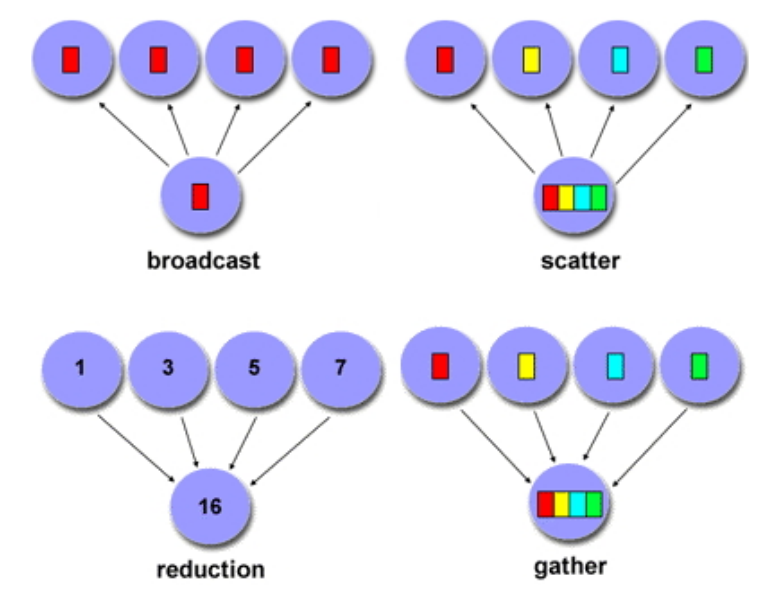
\includegraphics[width=6.0cm]{graphs/collectives.png}
 \end{figure}

\end{frame}


\subsection{Broadcast: Lab4}
\begin{frame}[fragile]
  \frametitle{Collectives: Broadcast: Lab4}
\begin{itemize}
\item A process has data that needs to be shared with all the others. For example:
\begin{itemize}
\item Process 0 parses command line arguments
\item Process 0 reads input file
\end{itemize}
\item {\color{mycolorcode}\verb|MPI_Bcast|} needs to be executed on all the processes
{\color{mycolorcode}
\begin{verbatim}
  int MPI_Bcast(void* buffer, int count, 
    MPI_Datatype datatype, 
    int root, MPI_Comm comm)
\end{verbatim}
}
here {\color{mycolorcode}\verb|root|} is the rank of the process that sends data
\end{itemize}
\end{frame}

\subsection{Scatter: Lab5}
\begin{frame}[fragile]
  \frametitle{Collectives: Scatter: Lab5}
\begin{itemize}
\item A process has an array {\color{mycolorcode}\verb|sendbuf|} that should be divided into subarrays of {\color{mycolorcode}\verb|sendcount|} elements which are sent into {\color{mycolorcode}\verb|recvbuf|} on each process:
{\color{mycolorcode}
\begin{verbatim}
  int MPI_Scatter(const void* sendbuf, int sendcount, 
    MPI_Datatype sendtype, void* recvbuf, 
    int recvcount, MPI_Datatype recvtype, int root,
    MPI_Comm comm)
\end{verbatim}
}
\end{itemize}
\end{frame}

\subsection{Scatterv}
\begin{frame}[fragile]
  \frametitle{Collectives: Scatterv}
\begin{itemize}
\item There is version of scatter that gives more control over which part of {\color{mycolorcode}\verb|sendbuf|} sent where
{\color{mycolorcode}
\begin{verbatim}
  int MPI_Scatterv(const void* sendbuf, 
    const int sendcounts[], const int displs[], 
    MPI_Datatype sendtype, void* recvbuf, 
    int recvcount, MPI_Datatype recvtype, 
    int root, MPI_Comm comm)
\end{verbatim}
}
Here {\color{mycolorcode}\verb|sendcounts|} and {\color{mycolorcode}\verb|displs|} specify how many elements from which location in {\color{mycolorcode}\verb|sendbuf|} to send to the processes
\end{itemize}
\end{frame}



\subsection{Gather: Lab5}
\begin{frame}[fragile]
  \frametitle{Collectives: Gather: Lab5}
\begin{itemize}
\item A process needs to collect into a single array {\color{mycolorcode}\verb|recvbuf|} arrays of {\color{mycolorcode}\verb|sendcount|} elements from all the processes
{\color{mycolorcode}
\begin{verbatim}
  int MPI_Gather(const void* sendbuf, int sendcount, 
    MPI_Datatype sendtype, void* recvbuf, 
    int recvcount, MPI_Datatype recvtype, int root,
    MPI_Comm comm)
\end{verbatim}
}
where {\color{mycolorcode}\verb|root|} is a rank of the receiving process
\end{itemize}
\end{frame}

\subsection{Gatherv}
\begin{frame}[fragile]
  \frametitle{Collectives: Gatherv}
\begin{itemize}
\item There is a version of gather that allows more control over how many elements are received from each process and where they are inserted into the {\color{mycolorcode}\verb|recvbuf|}
{\color{mycolorcode}
\begin{verbatim}
  int MPI_Gatherv(const void* sendbuf, int sendcount, 
    MPI_Datatype sendtype, void* recvbuf, 
    const int recvcounts[], const int displs[],
    MPI_Datatype recvtype, int root, MPI_Comm comm)
\end{verbatim}
}
Here 
\begin{itemize}
\item {\color{mycolorcode}\verb|recvcounts|} is an array of non-negative integers containing the number of elements received from each process
\item {\color{mycolorcode}\verb|displs|} an array of indexes where to put received data into {\color{mycolorcode}\verb|recvbuf|}.
\end{itemize}
\end{itemize}
\end{frame}

\subsection{Allgather}
\begin{frame}[fragile]
  \frametitle{Collectives: Allgather}
\begin{itemize}
\item It might be necessary to distribute gathered result to all the nodes. Instead of doing two separate calls, gather and broadcast, it is more efficient to use
{\color{mycolorcode}
\begin{verbatim}
  int MPI_Allgather(const void* sendbuf, int sendcount,
    MPI_Datatype sendtype, void* recvbuf, int recvcount,
    MPI_Datatype recvtype, MPI_Comm comm)
\end{verbatim}
}
\end{itemize}
\end{frame}

\subsection{Alltoall}
\begin{frame}[fragile]
  \frametitle{Collectives: Alltoall}
\begin{itemize}
\item {\color{mycolorcode}\verb|MPI_Alltoall|} is an extension of {\color{mycolorcode}\verb|MPI_Allgather|} to the case where each process
sends distinct data to each of the receivers. The j-th block sent from process i is received
by process j and is placed in the i-th block of {\color{mycolorcode}\verb|recvbuf|}.
{\color{mycolorcode}
\begin{verbatim}
  int MPI_Alltoall(const void* sendbuf, int sendcount, 
    MPI_Datatype sendtype, void* recvbuf, int recvcount, 
    MPI_Datatype recvtype, MPI_Comm comm)
\end{verbatim}
}
\end{itemize}
\end{frame}


\subsection{Reduce: Lab6}
\begin{frame}[fragile]
  \frametitle{Collectives: Reduce: Lab6}
\begin{itemize}
\item Reduce aggregates data from all the processes into sum, product, maximum, minimum, minloc, maxloc, and, or, etc:
{\color{mycolorcode}
\begin{verbatim}
  int MPI_Reduce(const void* sendbuf, void* recvbuf, 
    int count, MPI_Datatype datatype, MPI_Op op, 
    int root, MPI_Comm comm)
\end{verbatim}
}
\item On root rank, one can use {\color{mycolorcode}\verb|MPI_IN_PLACE|} instead of {\color{mycolorcode}\verb|sendbuf|} to avoid allocating two buffers but reuse {\color{mycolorcode}\verb|recvbuf|} to return the result of reduce in place
\item One can define custom aggregation operation:
{\color{mycolorcode}
\begin{verbatim}
  int MPI_Op_create(MPI_User_function* user_fn, 
    int commute, MPI_Op* op)
\end{verbatim}
}
\item The user-defined operation is assumed to be associative. 
\end{itemize}
\end{frame}

\begin{frame}[fragile]
  \frametitle{Collectives: Reduce: Lab6}
\begin{itemize}
\item The argument {\color{mycolorcode}\verb|user_fn|} is the user-defined function of the following type:
{\color{mycolorcode}
\begin{verbatim}
  typedef void MPI_User_function(void *invec, 
    void *inoutvec, int *len, MPI_Datatype *datatype)
\end{verbatim}
}
where 
{\color{mycolorcode}
\begin{verbatim}
  inoutvec[i] = invec[i] op inoutvec[i], i = 1..len-1
\end{verbatim}
}
\item After the user defined operation is used, it should be deallocated:
{\color{mycolorcode}
\begin{verbatim}
  int MPI_Op_free(MPI_Op *op)
\end{verbatim}
} 
\end{itemize}

\end{frame}

\subsection{Allreduce}
\begin{frame}[fragile]
  \frametitle{Collectives: Allreduce}
\begin{itemize}
\item There is a modification of reduce where each process gets aggregated value:
{\color{mycolorcode}
\begin{verbatim}
  int MPI_Allreduce(const void* sendbuf, void* recvbuf, 
    int count, MPI_Datatype datatype,  MPI_Op op, 
    MPI_Comm comm)
\end{verbatim}
}
\item It is faster then doing two operations: reduce and broadcast
\item There is also {\color{mycolorcode}\verb|MPI_Reduce_scatter|} available
\end{itemize}
\end{frame}


\subsection{Scan}
\begin{frame}[fragile]
  \frametitle{Collectives: Scan}
\begin{itemize}
\item If process $i$ contains a number $x_i$ and $\oplus$ is the operation, then the {\color{mycolordef}\textbf{inclusive scan}} operation leaves $x_0 \oplus ... \oplus x_i$ on processor $i$
{\color{mycolorcode}
\begin{verbatim}
  int MPI_Scan(const void* sendbuf, void* recvbuf, 
    int count, MPI_Datatype datatype, MPI_Op op, 
    MPI_Comm comm)
\end{verbatim}
}
\item An {\color{mycolordef}\textbf{exclusive scan}} operation leaves  $x_0 \oplus x_i$ on processor $i$ and its result is undefined on processor $0$
{\color{mycolorcode}
\begin{verbatim}
  int MPI_Exscan(const void* sendbuf, void* recvbuf, 
    int count, MPI_Datatype datatype, MPI_Op op, 
    MPI_Comm comm)
\end{verbatim}
}
\end{itemize}
\end{frame}

\subsection{Barrier}
\begin{frame}[fragile]
  \frametitle{Collectives: Barrier}
\begin{itemize}
\item The call blocks until all the processes reached it
{\color{mycolorcode}
\begin{verbatim}
  int MPI_Barrier(MPI_Comm comm)
\end{verbatim}
}
\item It is almost never necessary to synchronize processes through a barrier: for most purposes it does not matter if processes are out of sync. Conversely, collectives introduce a barrier of sorts themselves.
\end{itemize}
\end{frame}

\subsection{Non-blocking collective operations}
\begin{frame}[fragile]
  \frametitle{Collectives: non-blocking collective operations}

There are non-blocking versions of collective operations: 
\begin{itemize}
\item {\color{mycolorcode}\verb|MPI_Ibcast|}
\item {\color{mycolorcode}\verb|MPI_Igather|}, {\color{mycolorcode}\verb|MPI_Igatherv|}
\item {\color{mycolorcode}\verb|MPI_Iscatter|}, {\color{mycolorcode}\verb|MPI_Iscatterv|}
\item {\color{mycolorcode}\verb|MPI_Iallgather|}, {\color{mycolorcode}\verb|MPI_Iallgatherv|}
\item {\color{mycolorcode}\verb|MPI_Ialltoall|}, {\color{mycolorcode}\verb|MPI_Ialltoallv|}
\item {\color{mycolorcode}\verb|MPI_Ireduce|}, {\color{mycolorcode}\verb|MPI_Iallreduce|}
\item {\color{mycolorcode}\verb|MPI_Iscan|}, {\color{mycolorcode}\verb|MPI_Iexscan|}
\end{itemize}
\end{frame}


\begin{frame}[fragile]
  \frametitle{Collectives}
 \begin{figure}[h]
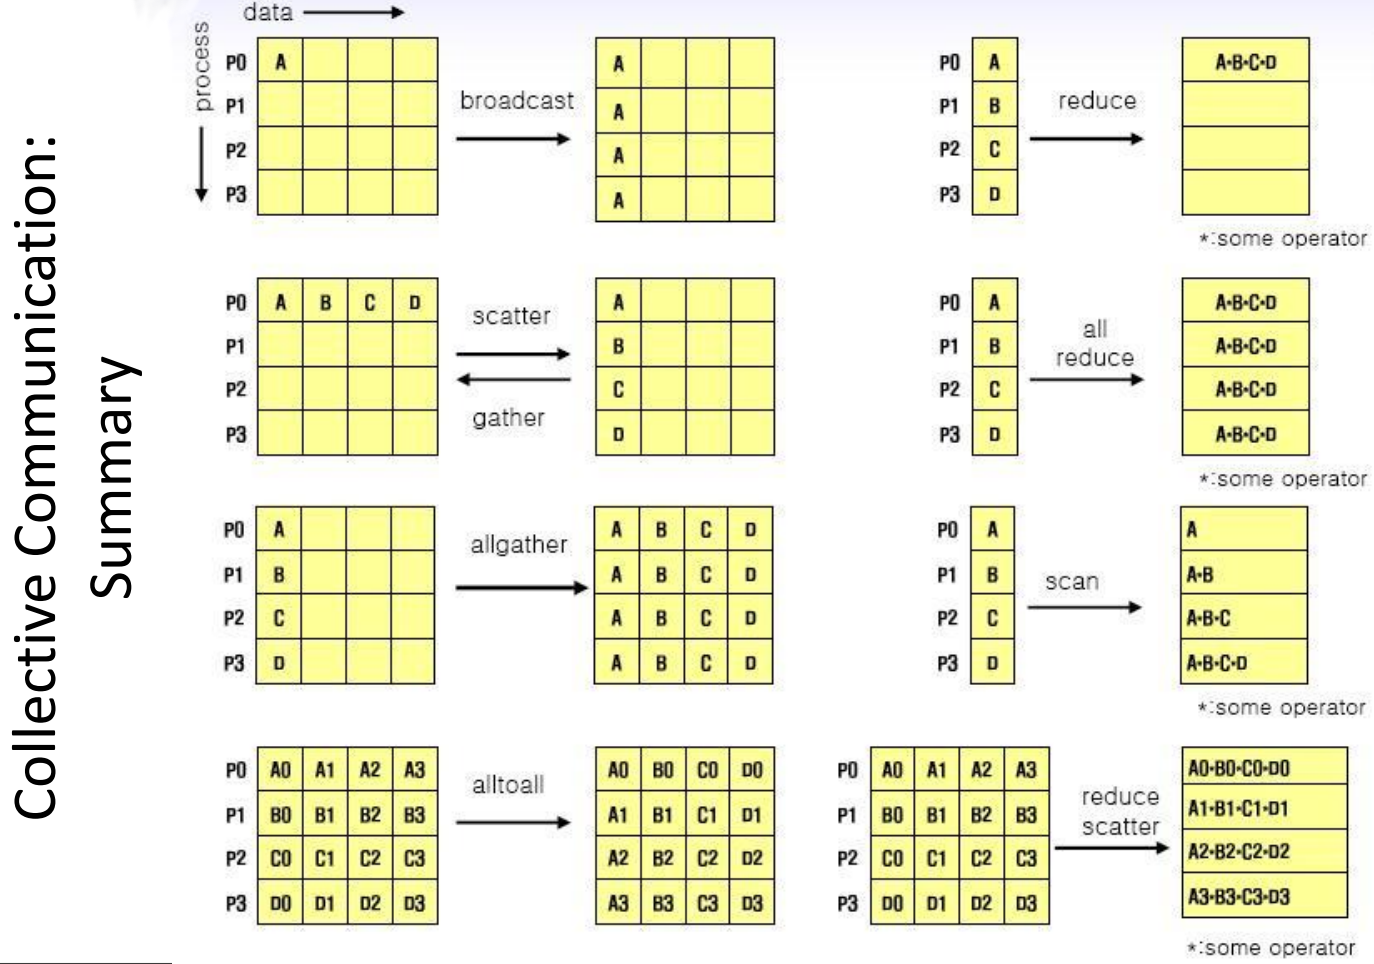
\includegraphics[width=11.0cm]{graphs/collectives1.png}
 \end{figure}

\end{frame}


\section{MPI data types}
\subsection{Elementary}
\begin{frame}[fragile]
  \frametitle{MPI data types: elementary}
\begin{itemize}
\item So far we were sending contiguous buffer with elements of a single type:
{\color{mycolorcode}
\begin{verbatim}
MPI_CHAR, MPI_UNSIGNED_CHAR, MPI_SIGNED_CHAR
MPI_SHORT, MPI_UNSIGNED_SHORT
MPI_INT
MPI_UNSIGNED
MPI_LONG, MPI_UNSIGNED_LONG
MPI_FLOAT
MPI_DOUBLE
MPI_LONG_DOUBLE
\end{verbatim}
}
\item MPI allows creating your own types that are not contiguous or are composite. Those are called {\color{mycolordef}\textbf{derived}}.
\end{itemize}
\end{frame}

\subsection{Derived: vector: Lab7}
\begin{frame}[fragile]
  \frametitle{MPI data types: derived: vector: Lab7}
  \begin{itemize}
  \item {\color{mycolorcode}\verb|MPI_Type_vector|} describes a series of blocks, all of equal size, spaced with a constant stride
{\color{mycolorcode}
\begin{verbatim}
  int MPI_Type_vector(int count, int blocklength, 
    int stride, MPI_Datatype oldtype, 
    MPI_Datatype *newtype)
\end{verbatim}
}
\item In the next example a vector type is created only on the sender, in order to send a strided subset of an array; the
  receiver receives the data as a contiguous block.
\end{itemize}
\begin{multicols}{2}
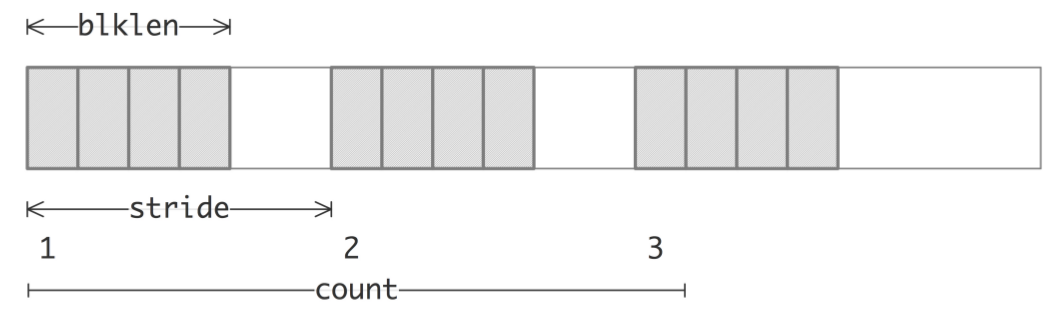
\includegraphics[width=6.0cm]{graphs/vector.png}
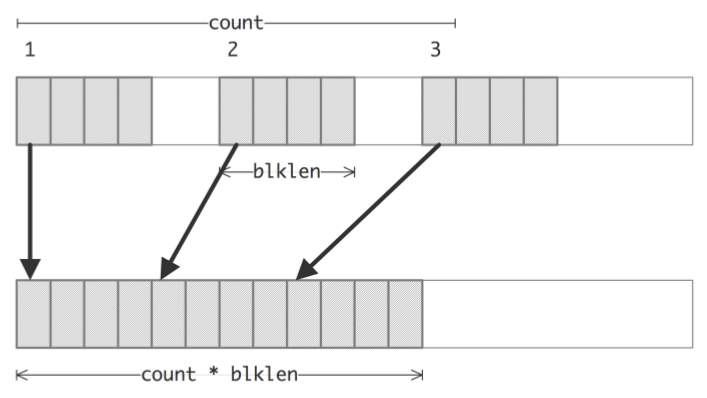
\includegraphics[width=6.0cm]{graphs/vector1.png}
\end{multicols}
\end{frame}


\begin{frame}[fragile]
  \frametitle{MPI data types: derived: vector}
{\color{mycolorcode}
\begin{verbatim}
  source = (double*) malloc(stride*count*sizeof(double));
  target = (double*) malloc(count*sizeof(double));
  MPI_Datatype newvectortype;
  if (procno==sender) {
    MPI_Type_vector(count,1,stride,MPI_DOUBLE,&newvectortype);
    MPI_Type_commit(&newvectortype);
    MPI_Send(source,1,newvectortype,the_other,0,comm);
    MPI_Type_free(&newvectortype);
  } else if (procno==receiver) {
    MPI_Status recv_status;
    int recv_count;
    MPI_Recv(target,count,MPI_DOUBLE,the_other,0,comm,
             &recv_status);
    MPI_Get_count(&recv_status,MPI_DOUBLE,&recv_count);
    ASSERT(recv_count==count);
}
\end{verbatim}
}
\end{frame}


\subsection{Derived: subarray}
\begin{frame}[fragile]
  \frametitle{MPI data types: derived: subarray}
\begin{itemize}
\item The vector datatype can be used for example, for cutting out blocks in an array of dimension 2. 
\item It still can be used recursively for higher dimensions but it gets tedious. Instead, there is an explicit subarray type:
{\color{mycolorcode}
\begin{verbatim}
  int MPI_Type_create_subarray(int ndims, 
    const int array_of_sizes[],
    const int array_of_subsizes[], 
    const int array_of_starts[], int order, 
    MPI_Datatype oldtype, MPI_Datatype *newtype)
\end{verbatim}
}
\begin{itemize}
\item {\color{mycolorcode}\verb|array_of_sizes|} - dimensions of full {\color{mycolorcode}\verb|ndims|}-array, 
\item {\color{mycolorcode}\verb|array_of_subsizes|} - dimensions of a subarray which starts at {\color{mycolorcode}\verb|array_of_starts|}
\end{itemize}
\end{itemize}
\end{frame}

\subsection{Derived: indexed: Lab7}
\begin{frame}[fragile]
  \frametitle{MPI data types: derived: indexed: Lab7}
\begin{itemize}
\item The indexed datatype can send arbitrary located elements from an array of a single datatype:
{\color{mycolorcode}
\begin{verbatim}
  int MPI_Type_indexed(int count, 
    const int array_of_blocklengths[],
    const int array_of_displacements[], 
    MPI_Datatype oldtype, MPI_Datatype *newtype)
\end{verbatim}
}
    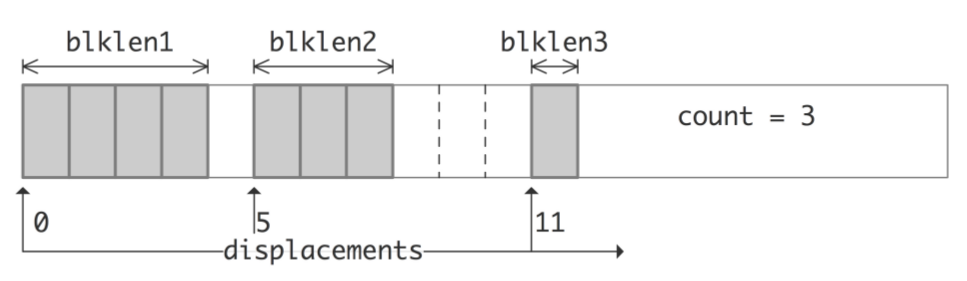
\includegraphics[width=8.0cm]{graphs/indexed.png}
\item There is also {\color{mycolorcode}\verb|MPI_Type_create_hindexed|} that measures index locations in bytes, rather than multiples of the old type.
\end{itemize}
\end{frame}

\subsection{Derived: struct: Lab7}
\begin{frame}[fragile]
  \frametitle{MPI data types: derived: struct: Lab7}
\begin{itemize}
\item The structure type can contain multiple data types. 
{\color{mycolorcode}
\begin{verbatim}
  int MPI_Type_create_struct(int count, 
    int blocklengths[], MPI_Aint displacements[],
    MPI_Datatype types[], MPI_Datatype *newtype);
\end{verbatim}
}
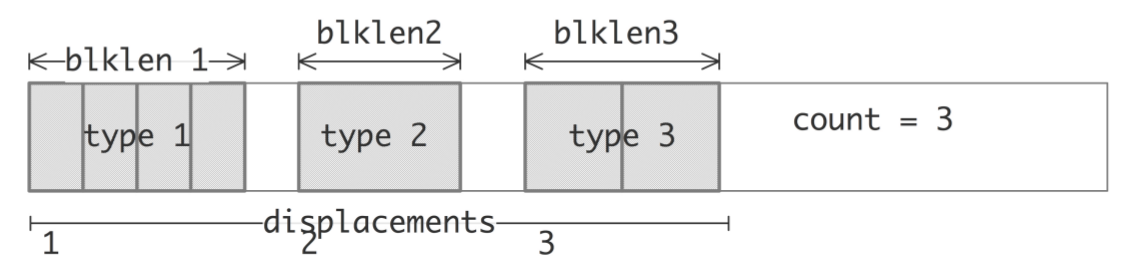
\includegraphics[width=10.0cm]{graphs/struct.png}
\end{itemize}
\end{frame}

\begin{frame}[fragile]
  \frametitle{MPI data types: derived: struct}
{\color{mycolorcode}
{\small
\begin{verbatim}
  struct object {
    char c;
    double x[2];
    int i;
  };
  MPI_Datatype newstructuretype;
  int structlen = 3;
  int blocklengths[structlen]; 
  MPI_Datatype types[structlen];
  MPI_Aint displacements[structlen];
  blocklengths[0] = 1; types[0] = MPI_CHAR;
  displacements[0] = (size_t)&(myobject.c) - (size_t)&myobject;
  blocklengths[1] = 2; types[1] = MPI_DOUBLE;
  displacements[1] = (size_t)&(myobject.x[0]) - (size_t)&myobject;
  blocklengths[2] = 1; types[2] = MPI_INT;
  displacements[2] = (size_t)&(myobject.i) - (size_t)&myobject;
\end{verbatim}
}
}
\end{frame}

\begin{frame}[fragile]
  \frametitle{MPI data types: derived: struct}
{\color{mycolorcode}
\begin{verbatim}
  MPI_Type_create_struct(structlen, blocklengths, 
    displacements, types, &newstructure);
  MPI_Type_commit(&newstructuretype);
  {
    MPI_Aint typesize;
    MPI_Type_extent(newstructuretype,&typesize);
    if(procno==0) 
      printf("Type extent: %d bytes\n",typesize);
  }
  if (procno==sender) {
    MPI_Send(&myobject,1,newstructuretype,the_other,0,comm);
  } else if (procno==receiver) {
    MPI_Recv(&myobject,1,newstructuretype,the_other,0,comm,
             MPI_STATUS_IGNORE)
  }
  MPI_Type_free(&newstructuretype);
\end{verbatim}
}
\end{frame}

\subsection{Derived: contiguous}
\begin{frame}[fragile]
  \frametitle{MPI data types: derived: contiguous}
\begin{itemize}
\item There is also a contiguos data type:
{\color{mycolorcode}
\begin{verbatim}
  int MPI_Type_contiguous(int count, 
    MPI_Datatype oldtype, MPI_Datatype *newtype)
\end{verbatim}
}
\item At first glance, there is no difference between using an array of elementary data types and contiguous type. 
\item The main reason to use contiguous type is to overcome a limitation on how many elements can be in the array of elementary data types ({\color{mycolorcode}\verb|MPI_int|} allows $2^{31}-1$ elements): 
to send more data one can use an array of contiguous data types instead.
\end{itemize}
\end{frame}


\section{Communicators}
\begin{frame}[fragile]
  \frametitle{Communicators}
\begin{itemize}
\item So far we have been using  {\color{mycolorcode}\verb|MPI_COMM_WORLD|} communicator that includes all the MPI processes requested by {\color{mycolorcli}\verb|mpirun|}
\item While only two processes communicate in send/receive operations, in collectives all the processes in the communicator talk to each other. This might be quite expensive for a program with millions of processes
\item Often there is a natural way to divide communication in the program into subgroups:
\begin{itemize}
\item Example 1. Simulation 
\begin{itemize}
\item inputs are generated
\item computations are performed on them
\item the results of the computations are analyzed and rendered graphically
\end{itemize}
Consider dividing your processes in three groups corresponding to generation, computation, rendering.
\item Example 2. You are doing some computation with a matrix and sometimes you need to make a collective calls only on a row/column (for example, to sum them with reduce). Create separate communicators for each row/column.
\end{itemize}
\end{itemize}
\end{frame}

\subsection{Split by color: Lab8}
\begin{frame}[fragile]
  \frametitle{Communicators: split by color: Lab8}
\begin{itemize}
\item One way to make processes to use different communicators it to use
{\color{mycolorcode}
\begin{verbatim}
  int MPI_Comm_split(MPI_Comm comm,
    int color, int key, MPI_Comm* newcomm)
\end{verbatim}
}
\item This is a collective call that runs on all the processes belonging to {\color{mycolorcode}\verb|comm|}. For each rank it computes {\color{mycolorcode}\verb|color|} and as a result ranks are divided into groups with the same color.
\item \verb|key| is used to decide how to sort ranks within the new communicator {\color{mycolorcode}\verb|newcomm|}. For example, if you use {\color{mycolorcode}\verb|comm|}'s rank as {\color{mycolorcode}\verb|key|}, 
the ranks within each {\color{mycolorcode}\verb|newcomm|} will preserve the same order as in the
original communicator
\item When creating separate communicator for each column in a matrix, use column number as color for a column to end up in the same communicator
\item After done using {\color{mycolorcode}\verb|newcomm|}, free it with {\color{mycolorcode}\verb|MPI_Comm_free|}.
\end{itemize}
\end{frame}

\begin{frame}[fragile]
  \frametitle{Communicators: split by color}
{\color{mycolorcode}
\begin{verbatim}
int world_rank, world_size;
MPI_Comm_rank(MPI_COMM_WORLD, &world_rank);
MPI_Comm_size(MPI_COMM_WORLD, &world_size);
int color = world_rank / 4; 
MPI_Comm row_comm;
MPI_Comm_split(MPI_COMM_WORLD, color, world_rank, &row_comm);
int row_rank, row_size;
MPI_Comm_rank(row_comm, &row_rank);
MPI_Comm_size(row_comm, &row_size);
printf("WORLD RANK/SIZE: %d/%d \t ROW RANK/SIZE: %d/%d\n",
	world_rank, world_size, row_rank, row_size);
MPI_Comm_free(&row_comm);
\end{verbatim}
}
\end{frame}

\subsection{Groups}
\begin{frame}[fragile]
  \frametitle{Communicators: groups}
\begin{itemize}
\item Internally MPI communicator has two parts:
\begin{itemize}
\item ID that differentiates one communicator from another
\item group of processes using the communicator
\end{itemize}
\item Using
{\color{mycolorcode}
\begin{verbatim}
  int MPI_Comm_group(MPI_Comm comm, MPI_Group* group)
\end{verbatim}
}
one can get {\color{mycolorcode}\verb|group|} object, then one can use the existing groups to create new groups that are union, intersection, subset, and finally one can create new communicator with the resulting group.
\end{itemize}
\end{frame}

\begin{frame}[fragile]
  \frametitle{Communicators: groups}
{\color{mycolorcode}
\begin{verbatim}
  int MPI_Group_union( MPI_Group group1, 
    MPI_Group group2, MPI_Group* newgroup)

  int MPI_Group_intersection(MPI_Group group1, 
    MPI_Group group2, MPI_Group* newgroup)

  int MPI_Group_incl(MPI_Group group, int n, 
    const int ranks[], MPI_Group* newgroup)

  int MPI_Comm_create_group(MPI_Comm comm, 
    MPI_Group group, int tag, MPI_Comm* newcomm)
\end{verbatim}
}
%If multiple threads at a given process perform concurrent
%{\color{mycolorcode}\verb|MPI_Comm_create_group|} operations, the user must distinguish these operations by
%providing different tag or comm arguments.
\end{frame}


\subsection{dup}
\begin{frame}[fragile]
  \frametitle{Communicators: dup}
\begin{itemize}
\item Suppose MPI program is using library that internally also uses MPI. 
\item Even if the program and the library operate on the same set of processes, one should use two different copies of communicators to avoid messages 
intended for your program to be mistakenly intercepted by a library or vice versa.
{\color{mycolorcode}
\begin{verbatim}
  int MPI_Comm_dup(MPI_Comm comm, 
      MPI_Comm *newcomm)
\end{verbatim}
}
\end{itemize}
\end{frame}

\subsection{Topology: Lab8}
\begin{frame}[fragile]
  \frametitle{Communicators: topology: Lab8}
\begin{itemize}
\item  In many parallel applications
a linear ranking of processes does not adequately reflect the logical communication pattern
of the processes
\item  Often the processes are logically arranged in n-dimensional grids, sometimes in a more general graph 
\item We call logical process arrangement of processes - ``virtual topology''.
\item A topology can provide a convenient naming mechanism for the processes
of a group 
\item Based on existing communicator with linear ranking, one can create a new communicator that in addition has topology information.
\item There are routines to query the topology of the communicator
\item For communicators with cartesian topology, there are routines to translate between linear and n-dimensional cartesian ranks
\item There are routines to find the neighbor in cartesian grid along certain dimension.
\item There are collectives that do data exchange between neighbors in virtual topology.
\end{itemize}
\end{frame}

\begin{frame}[fragile]
  \frametitle{Communicators: topology: cartesian: Lab8}
{\color{mycolorcode}
\begin{verbatim}
  int MPI_Cart_create(MPI_Comm comm_old, 
    int ndims, const int dims[],
    const int periods[], int reorder, 
    MPI_Comm *comm_cart)
\end{verbatim}
}
\begin{itemize}
\item {\color{mycolorcode}\verb|ndims|} - number of dimensions of Cartesian grid
\item {\color{mycolorcode}\verb|dims|} - integer array of size {\color{mycolorcode}\verb|ndims|} specifying the number of
processes in each dimension
\item {\color{mycolorcode}\verb|periods|} - logical array of size ndims specifying whether the grid
is periodic (true) or not (false) in each dimension
\item {\color{mycolorcode}\verb|reorder|} - ranking may be reordered (true) or not (false)
\end{itemize}
\end{frame}

\begin{frame}[fragile]
  \frametitle{Communicators: topology: cartesian: Lab8}
\begin{itemize}
\item One can query the topology to find parameters of the cartesian grid and translate between linear rank and cartesian coordinates
\end{itemize}
{\color{mycolorcode}
\begin{verbatim}
  int MPI_Cartdim_get(MPI_Comm comm, int *ndims)

  int MPI_Cart_get(MPI_Comm comm, int maxdims, 
    int dims[], int periods[], int coords[])

  int MPI_Cart_rank(MPI_Comm comm, const int coords[], 
    int *rank)

  int MPI_Cart_coords(MPI_Comm comm, int rank, 
    int maxdims, int coords[])
\end{verbatim}
}
here {\color{mycolorcode}\verb|coords|} are coordinates of the calling process
\end{frame}

\begin{frame}[fragile]
  \frametitle{Communicators: topology: cartesian: Lab8}
\begin{itemize}
\item One can find neighbors on the grid or in a graph:
{\color{mycolorcode}
\begin{verbatim}
  int MPI_Graph_neighbors_count(MPI_Comm comm, int rank, 
    int *nneighbors)

  int MPI_Graph_neighbors(MPI_Comm comm, int rank, 
    int maxneighbors, int neighbors[])
\end{verbatim}
}
\item If the process topology is a Cartesian structure, an {\color{mycolorcode}\verb|MPI_SENDRECV|} operation may be used
along a coordinate direction to perform a shift of data. As input, {\color{mycolorcode}\verb|MPI_SENDRECV|} takes
the rank of a source process for the receive, and the rank of a destination process for the
send. To get this information, call
{\color{mycolorcode}
\begin{verbatim}
  int MPI_Cart_shift(MPI_Comm comm, int direction, 
    int disp, int *rank_source, int *rank_dest)
\end{verbatim}
}
shift {\color{mycolorcode}disp} units along dimension {\color{mycolorcode}direction}
\end{itemize}
\end{frame}

\begin{frame}[fragile]
  \frametitle{Communicators: topology: cartesian: Lab8}
\begin{itemize}
\item One can partition cartesian space into subspaces:
\end{itemize}
{\color{mycolorcode}
\begin{verbatim}
  int MPI_Cart_sub(MPI_Comm comm, 
    const int remain_dims[], MPI_Comm *newcomm)
\end{verbatim}
}
\end{frame}

\begin{frame}[fragile]
  \frametitle{Communicators: topology: cartesian: collectives}
\begin{itemize}
\item Neighborhood gather:
{\color{mycolorcode}
\begin{verbatim}
  int MPI_Neighbor_allgather(const void* sendbuf, 
    int sendcount, MPI_Datatype sendtype,  void* recvbuf, 
    int recvcount, MPI_Datatype recvtype, MPI_Comm comm)
\end{verbatim}
}
\item In this function, each process i gathers data items from each process j if an edge (j, i) exists
in the topology graph, and each process i sends the same data items to all processes j where
an edge (i, j) exists. The send buffer is sent to each neighboring process and the l-th block
in the receive buffer is received from the l-th neighbor.
\end{itemize}
\end{frame}

\begin{frame}[fragile]
  \frametitle{Communicators: topology: cartesian: collectives}
\begin{itemize}
\item The vector version of gather allows to get different number of elements from different neighbors:
{\color{mycolorcode}
\begin{verbatim}
  int MPI_Neighbor_allgatherv(const void* sendbuf, 
    int sendcount, MPI_Datatype sendtype, 
    void* recvbuf, const int recvcounts[],
    const int displs[], MPI_Datatype recvtype, 
    MPI_Comm comm)
\end{verbatim}
}
\item {\color{mycolorcode}\verb|recvcounts|} - Non-negative integer array (of length indegree) containing
the number of elements that are received from
each neighbor
\item {\color{mycolorcode}\verb|displs|} - Integer array (of length indegree). Entry i specifies the
displacement (relative to {\color{mycolorcode}\verb|recvbuf|}) at which to place the
incoming data from neighbor i.
\end{itemize}
\end{frame}

\begin{frame}[fragile]
  \frametitle{Communicators: topology: cartesian: collectives}
\begin{itemize}
\item In this function, each process i receives data items from each process j if an edge (j, i)
exists in the topology graph or Cartesian topology. Similarly, each process i sends data
items to all processes j where an edge (i, j) exists. This call is more general than
{\color{mycolorcode}\verb|MPI_Neighbor_allgather|} in that different data items can be sent to each neighbor.
The k-th block in send buffer is sent to the k-th neighboring process and the l-th block in
the receive buffer is received from the l-th neighbor.
{\color{mycolorcode}
\begin{verbatim}
  int MPI_Neighbor_alltoall(const void* sendbuf, 
    int sendcount, MPI_Datatype sendtype, void* recvbuf, 
    int recvcount, MPI_Datatype recvtype, MPI_Comm comm)
\end{verbatim}
}
\item {\color{mycolorcode}\verb|MPI_Neighbor_alltoallv|} allows sending/receiving different
numbers of elements to and from each neighbor.
\item {\color{mycolorcode}\verb|MPI_Neighbor_alltoallw|} allows one to send and receive with different data types
to and from each neighbor.
\item Non-blocking neighbor collectives... Collectives for graphs...
\end{itemize}
\end{frame}

\subsection{Inter-communicators}
\begin{frame}[fragile]
  \frametitle{Communicators: inter-communicators}
\begin{itemize}
\item If two disjoint communicators exist, it may be necessary to communicate between them.
\item {\color{mycolorcode}\verb|MPI_Intercomm_create|} is used to bind two intra-communicators into an {\color{mycolordef}\textbf{inter-communicator}}
\item {\color{mycolorcode}\verb|MPI_Intercomm_merge|} creates an intra-communicator by merging the local and remote groups of an inter-communicator
\item Overlap of local and remote groups that are bound into an inter-communicator is
prohibited. 
\item The function {\color{mycolorcode}\verb|MPI_Intercomm_create|} can be used to create an inter-communicator
from two existing intra-communicators, in the following situation: At least one selected
member from each group (the “group leader”) has the ability to communicate with the
selected member from the other group; that is, a “peer” communicator exists to which both
leaders belong, and each leader knows the rank of the other leader in this peer communicator.
Furthermore, members of each group know the rank of their leader.
\end{itemize}
\end{frame}

\begin{frame}[fragile]
  \frametitle{Communicators: inter-communicators}
{\color{mycolorcode}
\begin{verbatim}
  int MPI_Intercomm_create(MPI_Comm local_comm, 
    int local_leader, MPI_Comm peer_comm, 
    int remote_leader, int tag,
    MPI_Comm *newintercomm)
\end{verbatim}
}
\begin{itemize}
\item This call creates an inter-communicator. 
\item It is collective over the union of the local and
remote groups. 
\item Processes should provide identical {\color{mycolorcode}\verb|local_comm|} and {\color{mycolorcode}\verb|local_leader|} arguments
within each group
\item After this, the intercommunicator can be used in collectives.
\end{itemize}
\end{frame}

\begin{frame}[fragile]
  \frametitle{Communicators: inter-communicators}
{\color{mycolorcode}
\begin{verbatim}
  int MPI_Intercomm_merge(MPI_Comm intercomm, 
    int high, MPI_Comm *newintracomm)
\end{verbatim}
}
\begin{itemize}
\item This function creates an intra-communicator from the union of the two groups that are
associated with intercomm.
\item All processes should provide the same high value within each
of the two groups. 
\item If processes in one group provided the value $high = false$ and processes
in the other group provided the value $high = true$ then the union orders the “low” group
before the “high” group. 
\item If all processes provided the same high argument then the order
of the union is arbitrary.
\item This call is blocking and collective within the union of the two
groups.
\end{itemize}
\end{frame}



\section{MPI-IO}

\subsection{Motivation}

\begin{frame}[fragile]
  \frametitle{MPI-IO: motivation}

\begin{itemize}
\item How to get the data from hundreds thousands of nodes on the cluster to disks?
\item I/O is much slower then computing and might become major bottleneck
\item Number of tasks keeps rising rapidly
\item The size of the data is also rapidly increasing
\item The gap between computational power and I/O rates keeps increasing
\item Letting each process write its own file and later gluing them all together? - Might be very inefficient if done on the same file system, overloads metadata server.
\item MPI-IO can often do it several hundered times faster by providing collective access to parallel file system (GPFS, Lustre, ...) and underlying storage hardware to all the processes in the communicator
\end{itemize}
\end{frame}


\subsection{Opening and closing files}
\begin{frame}[fragile]
  \frametitle{MPI-IO: opening and closing files}
{\color{mycolorcode}
\begin{verbatim}
  int MPI_File_open(MPI_Comm comm, const char *filename, 
    int amode, MPI_Info info, MPI_File *fh)
\end{verbatim}
}
\begin{itemize}
\item It is a collective routine: all the processes in the communicator must provide the same value for {\color{mycolorcode}\verb|amode|} and {\color{mycolorcode}\verb|filename|}
\item Some possible values for {\color{mycolorcode}\verb|amode|}:
{\color{mycolorcode}
\begin{itemize}
\item {\color{mycolorcode}\verb|MPI_MODE_RDONLY|} - read only
\item {\color{mycolorcode}\verb|MPI_MODE_RDWR|} - write only
\item {\color{mycolorcode} \verb|MPI_MODE_WRONLY|} - write only
\item {\color{mycolorcode}\verb|MPI_MODE_CREATE|} - create the file if it does not exist
\item {\color{mycolorcode}\verb|MPI_MODE_SEQUENTIAL|} - file will only be accessed sequentially
\end{itemize}
}
\item Via {\color{mycolorcode}\verb|info|} object one can provide hints to help to optimize I/O, {\color{mycolorcode}\verb|MPI_INFO_NULL|} - no hints, hints are implementation and hardware specific 
\item The output of the call is the file handle {\color{mycolorcode}\verb|fh|}
\item The file is closed with
{\color{mycolorcode}
\begin{verbatim}
int MPI_File_close(MPI_File *fh)
\end{verbatim}
}
\end{itemize}
\end{frame}

\subsection{File pointer: Lab9}
\begin{frame}[fragile]
  \frametitle{MPI-IO: file pointer: Lab9}
\begin{itemize}
\item Each process moves its local file pointer (individual file pointer) with
{\color{mycolorcode}
\begin{verbatim}
  int MPI_File_seek(MPI_File fh, MPI_Offset offset, 
    int whence)
\end{verbatim}
}
\item {\color{mycolorcode}\verb|whence|} can be
\begin{itemize}
\item {\color{mycolorcode}\verb|MPI_SEEK_SET|} - the pointer is set to {\color{mycolorcode}\verb|offset|} counting from the beginning of the file
\item {\color{mycolorcode}\verb|MPI_SEEK_CUR|} - the pointer is set to the current position plus {\color{mycolorcode}\verb|offset|}
\item {\color{mycolorcode}\verb|MPI_SEEK_END|} - the point is set to the end of file plus {\color{mycolorcode}\verb|offset|}
\end{itemize}
\item One can query the current position of the file pointer with
{\color{mycolorcode}
\begin{verbatim}
  int MPI_File_get_position(MPI_File fh, 
    MPI_Offset *offset)
\end{verbatim}
}
\item {\color{mycolorcode}\verb|MPI_Offset|} is an integer type of size sufficient to represent the size (in bytes) of the largest
file supported by MPI. Displacements and offsets are always specified as values of type
{\color{mycolorcode}\verb|MPI_Offset|}.
\end{itemize}
\end{frame}

\begin{frame}[fragile]
  \frametitle{MPI-IO: file pointer: Lab9}
\begin{itemize}
\item Read file at individual file pointer (can be different for different processes)
{\color{mycolorcode}
\begin{verbatim}
  int MPI_File_read(MPI_File fh, void *buf, 
    int count, MPI_Datatype datatype, MPI_Status *status)
\end{verbatim}
}
\item Updates position of file pointer after reading
\item Not thread safe
\item Similarly, one can write using individual file pointer:
{\color{mycolorcode}
\begin{verbatim}
  int MPI_File_write(MPI_File fh, const void *buf, 
    int count, MPI_Datatype datatype, MPI_Status *status)
\end{verbatim}
}
\end{itemize}
\end{frame}

\subsection{Explicit offset}
\begin{frame}[fragile]
  \frametitle{MPI-IO: explicit offset}
\begin{itemize}
\item Instead of using individual (per process) file pointers that get changed by read/write and are not thread safe, one can use explicit offsets:
{\color{mycolorcode}
\begin{verbatim}

  int MPI_File_read_at(MPI_File fh, MPI_Offset offset, 
    void *buf, int count, MPI_Datatype datatype, 
    MPI_Status *status)

  int MPI_File_write_at(MPI_File fh, MPI_Offset offset, 
    const void *buf, int count, MPI_Datatype datatype, 
    MPI_Status *status)

\end{verbatim}
}
\item Thread-safe
\item The file pointer is neither referred nor incremented
\end{itemize}
\end{frame}

\subsection{Collective and non-blocking operations}
\begin{frame}[fragile]
  \frametitle{MPI-IO: collective and non-blocking operations}
\begin{itemize}
\item I/O can be performed collectively by all processes in a
communicator
\begin{itemize}
\item {\color{mycolorcode}\verb|MPI_File_read_all|}
\item {\color{mycolorcode}\verb|MPI_File_write_all|}
\item {\color{mycolorcode}\verb|MPI_File_read_at_all|}
\item {\color{mycolorcode}\verb|MPI_File_write_at_all|}
\end{itemize}
\item Same parameters as in independent I/O functions
\item All processes in communicator that opened file must call
function
\item Performance potentially better than for individual
functions
\begin{itemize}
\item Even if each processor reads a non-contiguous segment, in
total the read is contiguous
\end{itemize}
\item There are also corresponding non-blocking functions that allow to overlap I/O with computations
\end{itemize}
\end{frame}

\subsection{Non-contiguous data access: fileview: Lab9}
\begin{frame}[fragile]
  \frametitle{MPI-IO: Non-contiguous data access: fileview: Lab9}
\begin{itemize}
\item By default, file is treated as consisting of bytes, and
process can access (read or write) any byte in the file
\item The {\color{mycolordef}fileview} defines which portion of a file is visible to a
process
\item A fileview consists of three components
\begin{itemize}
\item {\color{mycolorcode}\verb|displacement|}: number of bytes to skip from the beginning
of file
\item {\color{mycolorcode}\verb|etype|}: type of data accessed, defines unit for offsets
\item {\color{mycolorcode}\verb|filetype|}: portion of file visible to a process - can be non-contiguous like such datatypes as vector, indexed, subarray, etc.
\end{itemize}
{\color{mycolorcode}
\begin{verbatim}
  int MPI_File_set_view(MPI_File fh, MPI_Offset disp, 
    MPI_Datatype etype, MPI_Datatype filetype, 
    const char *datarep, MPI_Info info)
\end{verbatim}
}
\item {\color{mycolorcode}\verb|datarep|} - data representation, controls file portability vs performance
\end{itemize}
\end{frame}

\begin{frame}[fragile]
  \frametitle{MPI-IO: Non-contiguous data access: fileview: Lab9}
\begin{itemize}
\item MPI-IO writes data into a file in a binary format. Possible values for {\color{mycolorcode}\verb|datarep|}
\begin{itemize}
\item {\color{mycolorcode}native} - default; data is written to file exactly as it is stored in memory; best performance; might be non-portable between different hardware or MPI implementations
\item {\color{mycolorcode}internal} - portable for the same MPI implementation on different hardware; worse performance
\item {\color{mycolorcode}external32} - completely portable; possibly worse performance; possibly some loss in precision
\end{itemize}
\item Each process has to access small pieces of data scattered
throughout a file; this is controlled by {\color{mycolorcode}\verb|filetype|}, {\color{mycolorcode}\verb|displacement|} and {\color{mycolorcode}\verb|etype|} 
(in terms of which everything is measured). Here different processes write to subarrays of different colors scattered in the file:
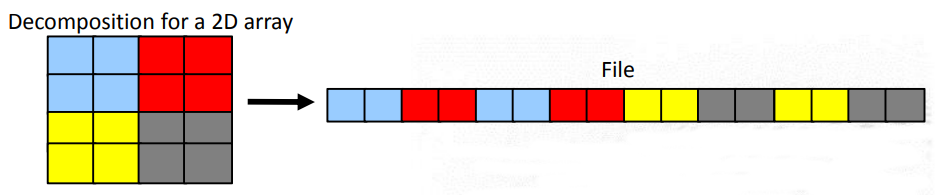
\includegraphics[width=8.0cm]{graphs/fileview.png}
\end{itemize}
\end{frame}

\begin{frame}[fragile]
  \frametitle{MPI-IO: Non-contiguous data access: fileview: Lab9}
\begin{itemize}
\item This would be very expensive if implemented with separate
reads/writes:
\begin{itemize}
\item I/O is done in blocks: the whole block has to be read from disk even if a small piece of data from it is required
\item Blocks are accessed sequentially to avoid race condition
\item If two different data items in the same block are needed by different processes, this would be done sequentially - false sharing
\item MPI-IO sees the whole picture and can read necessary blocks into memory and then send different pieces of it to different processes avoiding false sharing
\end{itemize}
\item If you do not use fileview, the data layout in a file would depend on the number of processes used in a job and you would have to do later some translation into a more portable format
\end{itemize}
\end{frame}

\subsection{HDF5: Lab10}
\begin{frame}[fragile]
  \frametitle{HDF5: Lab10}
\begin{itemize}
\item If you want to sacrifice some performance for a lot of convenience, you can use parallel version of HDF5 library that knows how to talk to MPI and do parallel I/O
\item The advantage is that you are working with a standard portable format for scientific computing that can be used in combination with many other tools and languages: ParaView, VisIt, python, C/C++, ROOT, etc.
\end{itemize}
\end{frame}

\subsection{T3PIO}
\begin{frame}[fragile]
  \frametitle{T3PIO}
\begin{itemize}
\item Some sites, for example TACC, developed libraries to provide reasonable hints to MPI-IO given the existing hardware.
\item The parallel I/O performance depends on three parameters:
\begin{itemize}
\item Number of writers
\item Number of stripes
\item Stripe size
\end{itemize}
\item T3IO library at TACC is claimed to be able to speed up MPI-IO by a factor of 10s by providing reasonable default parameters to Lustre file system
\item MPI-IO can take hints, if it was compiled with the support for the particular file system
\item The hints are passed via {\color{mycolorcode}\verb|info|} object in the form of key-value pairs. Those pairs that are not understood, are ignored. Also, even if the hints are understood, there is no guarantee that they will be used. 
It is implementation dependent.
\item Since parallel HDF5 is built on top of MPI-IO, T3PIO and hints in general might help it as well.
\end{itemize}
\end{frame}

\section{One-sided communication}
\subsection{Motivation}
\begin{frame}[fragile]
  \frametitle{One-sided communication: motivation}
\begin{itemize}
\item The basic idea of one-sided communication models is to
decouple data movement with process synchronization
\begin{itemize}
\item one should be able to move data without requiring that the remote
process synchronize
\item Each process exposes a part of its memory to other processes
\item Other processes can directly read from or write to this memory
\item Can do multiple data transfers with a single
synchronization operation
\end{itemize}
\item Some irregular communication patterns can be
more economically expressed
\item Can be significantly faster than send/receive
on systems with hardware support for remote
memory access (RMA)
\end{itemize}
\end{frame}


\subsection{Window}
\begin{frame}[fragile]
  \frametitle{One-sided communication: window}
\begin{itemize}
\item One can declare part of local memory, called {\color{mycolordef}\textbf{window}}, to be publically accessible in four ways:
\begin{enumerate}
\item You already have an allocated buffer that you
would like to make remotely accessible
{\color{mycolorcode}
\begin{verbatim}
  int MPI_Win_create(void *base, MPI_Aint size, 
    int disp_unit, MPI_Info info,
    MPI_Comm comm, MPI_Win *win)
\end{verbatim}
}
\begin{itemize}
\item {\color{mycolorcode}\verb|base|} - pointer to the existing buffer
\item {\color{mycolorcode}\verb|size|} - size of window in bytes
\item {\color{mycolorcode}\verb|disp_unit|} - local unit size for displacements, in bytes 
\end{itemize}
\item  You want to create a buffer and directly make it
remotely accessible. This is better since MPI might allocate data in a more optimal memory address for MPI communication. If the first option is used, use {\color{mycolorcode}\verb|MPI_alloc|} instead of malloc.
{\color{mycolorcode}
\begin{verbatim}
  int MPI_Win_allocate(MPI_Aint size, int disp_unit, 
    MPI_Info info, MPI_Comm comm, void *baseptr, 
    MPI_Win *win)
\end{verbatim}
}
\end{enumerate}
\end{itemize}
\end{frame}

\begin{frame}[fragile]
  \frametitle{One-sided communication: window}
\begin{itemize}
\item[]
\begin{enumerate}
\setcounter{enumi}{3}
\item You don’t have a buffer yet, but will have one in
the future
{\color{mycolorcode}
\begin{verbatim}
  int MPI_Win_create_dynamic(MPI_Info info, MPI_Comm comm, 
    MPI_Win *win)
\end{verbatim}
}
\begin{itemize}
\item Later you can use the following calls to attach/detach a buffer to/from the window:
{\color{mycolorcode}
\begin{verbatim}
  int MPI_Win_attach(MPI_Win win, void *base, 
    MPI_Aint size)
  int MPI_Win_detach(MPI_Win win, 
    const void *base)
\end{verbatim}
}
\end{itemize}
\item You want multiple processes on the same node
to share a buffer
{\color{mycolorcode}
\begin{verbatim}
  int MPI_Win_allocate_shared(MPI_Aint size, 
    int disp_unit, MPI_Info info, MPI_Comm comm, 
    void *baseptr, MPI_Win *win)
\end{verbatim}
}
\end{enumerate}

\item Window creation are collective calls executed on all the processes of the communicator
\item The buffer sizes can be different for different processes
\item To release the window, run on all the involved processes
{\color{mycolorcode}
\begin{verbatim}
  int MPI_Win_free(MPI_Win *win)
\end{verbatim}
}
\end{itemize}
\end{frame}


\subsection{Data movement}
\begin{frame}[fragile]
  \frametitle{One-sided communication: data movement}
\begin{itemize}
\item MPI provides ability to read, write
and atomically modify data in
remotely accessible memory
regions
\begin{itemize}
\item {\color{mycolorcode}\verb|MPI_Get|}
\item {\color{mycolorcode}\verb|MPI_Put|}
\item {\color{mycolorcode}\verb|MPI_Accumulate|}
\item {\color{mycolorcode}\verb|MPI_Get_accumulate|}
\item {\color{mycolorcode}\verb|MPI_Compare_and_swap|}
\item {\color{mycolorcode}\verb|MPI_Fetch_and_op|}
\end{itemize}
\item All data movement operations are non-blocking
\end{itemize}
\end{frame}

\subsection{Data movement: put}
\begin{frame}[fragile]
  \frametitle{One-sided communication: data movement: put}
\begin{itemize}
\item Move data from origin, to target
{\color{mycolorcode}
\begin{verbatim}
  int MPI_Put(const void *origin_addr, int origin_count,
    MPI_Datatype origin_datatype, int target_rank,
    MPI_Aint target_disp, int target_count,
    MPI_Datatype target_datatype, MPI_Win win)
\end{verbatim}
}
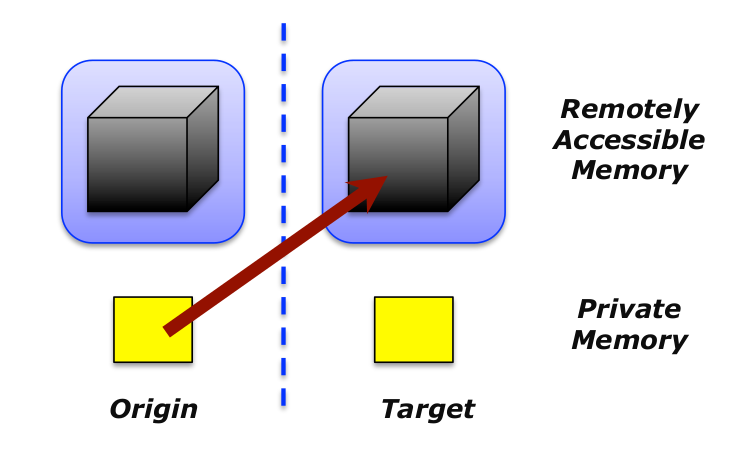
\includegraphics[width=6.0cm]{graphs/put.png}
\end{itemize}
\end{frame}

\subsection{Data movement: get}
\begin{frame}[fragile]
  \frametitle{One-sided communication: data movement: get}
\begin{itemize}
\item Move data to origin, from target
{\color{mycolorcode}
\begin{verbatim}
  int MPI_Get(void *origin_addr, int origin_count,
    MPI_Datatype origin_datatype, int target_rank,
    MPI_Aint target_disp, int target_count,
    MPI_Datatype target_datatype, MPI_Win win)
\end{verbatim}
}
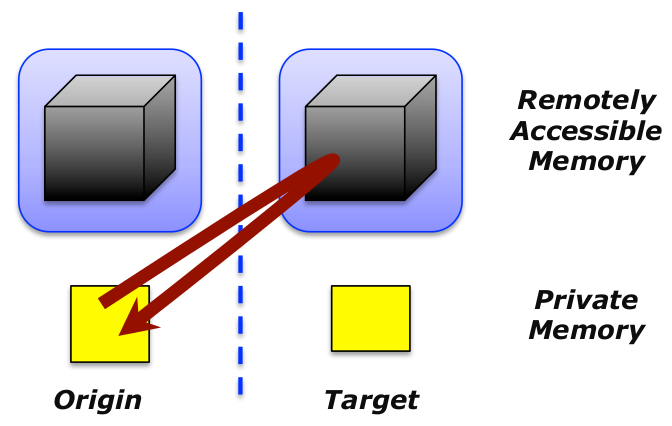
\includegraphics[width=6.0cm]{graphs/get.png}
\end{itemize}
\end{frame}

\subsection{Data movement: accumulate}
\begin{frame}[fragile]
  \frametitle{One-sided communication: data movement: accumulate}
\begin{itemize}
\item Element-wise atomic update operation, similar to a put
\begin{itemize}
\item Reduces origin and target data into target buffer using op
argument as combiner
\item Predefined ops only, no user-defined operations
\end{itemize}
{\color{mycolorcode}
\begin{verbatim}
  int MPI_Accumulate(const void *origin_addr, 
    int origin_count, MPI_Datatype origin_datatype, 
    int target_rank, MPI_Aint target_disp, 
    int target_count, MPI_Datatype target_datatype, 
    MPI_Op op, MPI_Win win)
\end{verbatim}
}
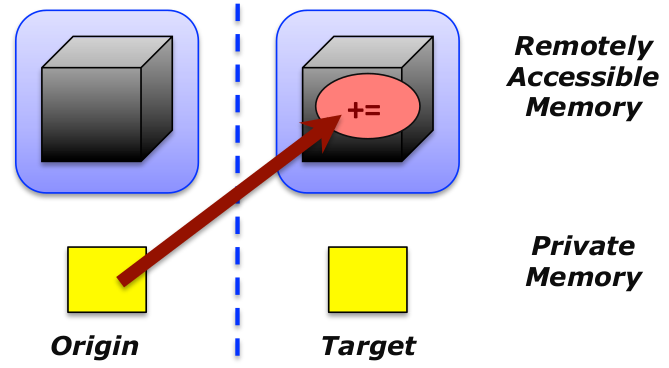
\includegraphics[width=5.0cm]{graphs/accumulate.png}
\item {\color{mycolorcode}\verb|Op = MPI_REPLACE|} corresponds to atomic put
\end{itemize}
\end{frame}

\subsection{Data movement: get accumulate}
\begin{frame}[fragile]
  \frametitle{One-sided communication: data movement: get accumulate}
\begin{itemize}
\item Element-wise atomic read-modify-write
\begin{itemize}
\item Op = {\color{mycolorcode}\verb|MPI_SUM|}, {\color{mycolorcode}\verb|MPI_PROD|}, {\color{mycolorcode}\verb|MPI_OR|}, {\color{mycolorcode}\verb|MPI_REPLACE|},
{\color{mycolorcode}\verb|MPI_NO_OP|}, ...
\end{itemize}
\item Result stored in target buffer
\item Original data stored in result buf on the origin node
\item Element-wise atomic get with {\color{mycolorcode}\verb|MPI_NO_OP|}
\item Element-wise atomic swap with {\color{mycolorcode}\verb|MPI_REPLACE|}
{\color{mycolorcode}
\begin{verbatim}
  int MPI_Get_accumulate(const void *origin_addr, 
    int origin_count, MPI_Datatype origin_datatype, 
    void *result_addr, int result_count, 
    MPI_Datatype result_datatype, int target_rank, 
    MPI_Aint target_disp, int target_count,
    MPI_Datatype target_datatype, MPI_Op op, MPI_Win win)
\end{verbatim}
}
\end{itemize}
\end{frame}

\subsection{Data movement: fetch and op}
\begin{frame}[fragile]
  \frametitle{One-sided communication: data movement: fetch and op }
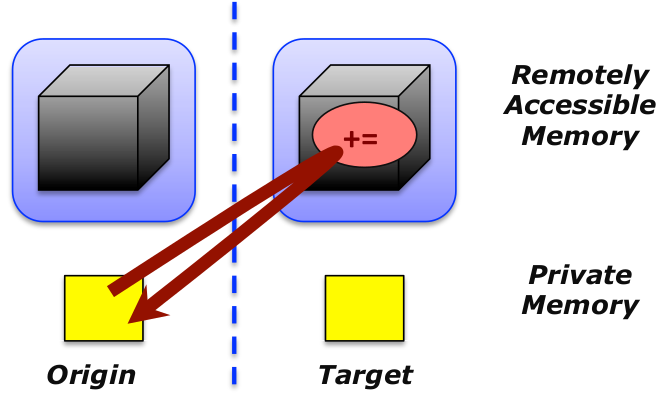
\includegraphics[width=6.0cm]{graphs/get_accumulate.png}
\begin{itemize}
\item {\color{mycolorcode}\verb|MPI_Fetch_and_op|} is a simpler version of {\color{mycolorcode}\verb|MPI_Get_accumulate|}:
\begin{itemize}
\item All buffers share a single predefined datatype
\item No count argument (it's always 1)
\item Simpler interface allows hardware optimization
\end{itemize}
{\color{mycolorcode}
\begin{verbatim}
  int MPI_Fetch_and_op(const void *origin_addr, 
    void *result_addr, MPI_Datatype datatype, 
    int target_rank, MPI_Aint target_disp,
    MPI_Op op, MPI_Win win)
\end{verbatim}
}
\end{itemize}
\end{frame}

\subsection{Data movement: compare and swap}
\begin{frame}[fragile]
  \frametitle{One-sided communication: data movement: compare and swap }
\begin{itemize}
\item 
Another useful operation is an atomic compare and swap where the value at the origin is
compared to the value at the target, which is atomically replaced by a third value only if
the values at origin and target are equal.
{\color{mycolorcode}
\begin{verbatim}
  int MPI_Compare_and_swap(const void *origin_addr, 
    const void *compare_addr, void *result_addr, 
    MPI_Datatype datatype, int target_rank,
    MPI_Aint target_disp, MPI_Win win)
\end{verbatim}
}
\end{itemize}
\end{frame}

\subsection{Ordering of operations}
\begin{frame}[fragile]
  \frametitle{One-sided communication: ordering of operations }
\begin{itemize}
\item  No guaranteed ordering for Put/Get operations
\item Result of concurrent Puts to the same location
undefined
\item Result of Get concurrent with Put/Accumulate undefined
\item Result of concurrent accumulate operations to the
same location are defined according to the order in
which the occurred
\item Remember that you can simulate atomic put and get:
\begin{itemize}
\item Atomic put: {\color{mycolorcode}\verb|Accumulate|} with {\color{mycolorcode}\verb|op = MPI_REPLACE|}
\item Atomic get: {\color{mycolorcode}\verb|Get_accumulate|} with {\color{mycolorcode}\verb|op = MPI_NO_OP|}
\end{itemize}
\end{itemize}
\end{frame}

\subsection{Synchronization models}
\begin{frame}[fragile]
  \frametitle{One-sided communication: synchronization models }
  \begin{itemize}
  \item RMA data access model
    \begin{itemize}
    \item When is a process allowed to read/write remotely accessible
      memory?
    \item When is data written by process X is available for process Y to read?
    \end{itemize}
  \item Three synchronization models provided by MPI:
    \begin{itemize}
    \item {\color{mycolordef}\textbf{Fence - active target synchronization}}
    \item {\color{mycolordef}\textbf{Post-start-complete-wait - generalized active target synchronization}}
    \item {\color{mycolordef}\textbf{Lock/Unlock - passive target synchronization}}
    \end{itemize}
  \item Data accesses occur within {\color{mycolordef}\textbf{epochs}}:
    \begin{itemize}
      \item {\color{mycolordef}\textbf{Access epochs}}: contain a set of operations issued by an origin process
      \item {\color{mycolordef}\textbf{Exposure epochs}}: enable remote processes to access and/or update a target's window
      \item Epochs define ordering and completion semantics
      \item Synchronization models provide mechanisms for establishing epochs
    \end{itemize}
  \end{itemize}
\end{frame}

\subsection{Synchronization models: fence}
\begin{frame}[fragile]
  \frametitle{One-sided communication: synchronization models: fence }
  \begin{itemize}
  \item Active target synchronization
  \item Collective synchronization model: starts and ends access and exposure epochs on all processes in the window
{\color{mycolorcode}
\begin{verbatim}
  int MPI_Win_fence(int assert, MPI_Win win)
\end{verbatim}
}
    \begin{itemize}
    \item The assert argument is used to provide assertions on the context of the call that may
      be used for various optimizations. A value of {\color{mycolorcode}\verb|assert = 0|} is always valid.
    \end{itemize}
  \item All processes in group of {\color{mycolorcode}\verb|win|} do an {\color{mycolorcode}\verb|MPI_Win_fence|} to open an epoch
  \item Everyone can issue put/get/accumulate operations to read/write data
  \item Everyone does an {\color{mycolorcode}\verb|MPI_Win_fence|} again to close the fence epoch
  \item All operations complete at the second fence synchronization
\end{itemize}
\end{frame}

\begin{frame}[fragile]
  \frametitle{One-sided communication: synchronization models: fence }
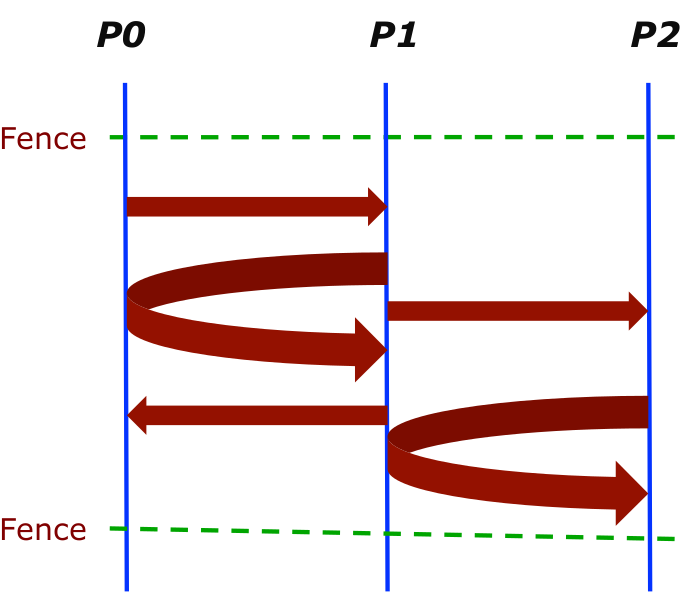
\includegraphics[width=6.0cm]{graphs/fence.png}
\end{frame}

\subsection{Synchronization models: PSCW}
\begin{frame}[fragile]
  \frametitle{One-sided communication: synchronization models: PSCW }
  \begin{itemize}
    \item PSCW = Post/Start/Complete/Wait
    \item Generalized Active Target Synchronization
    \item Like fence, but origin and target specify who they communicate with
\begin{multicols}{2}
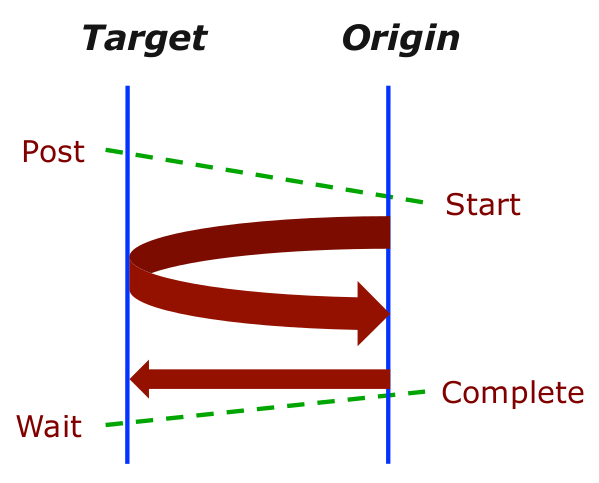
\includegraphics[width=6.0cm]{graphs/pscw.png}
{\color{mycolorcode}
{\tiny
\begin{verbatim}
  int MPI_Win_post(MPI_Group group, 
    int assert, MPI_Win win)

  int MPI_Win_start(MPI_Group group, 
    int assert, MPI_Win win)

  int MPI_Win_complete(MPI_Win win)

  int MPI_Win_wait(MPI_Win win)
\end{verbatim}
}
}
\begin{itemize}
\item All synchronization operations may block, to enforce P-S/C-W ordering
\item Processes can be both origins and targets
\end{itemize}
\end{multicols}
  \end{itemize}
\end{frame}

\subsection{Synchronization models: passive target}
\begin{frame}[fragile]
  \frametitle{One-sided communication: synchronization models: passive target}
  \begin{itemize}
  \item What if each process may need to independently access data?
    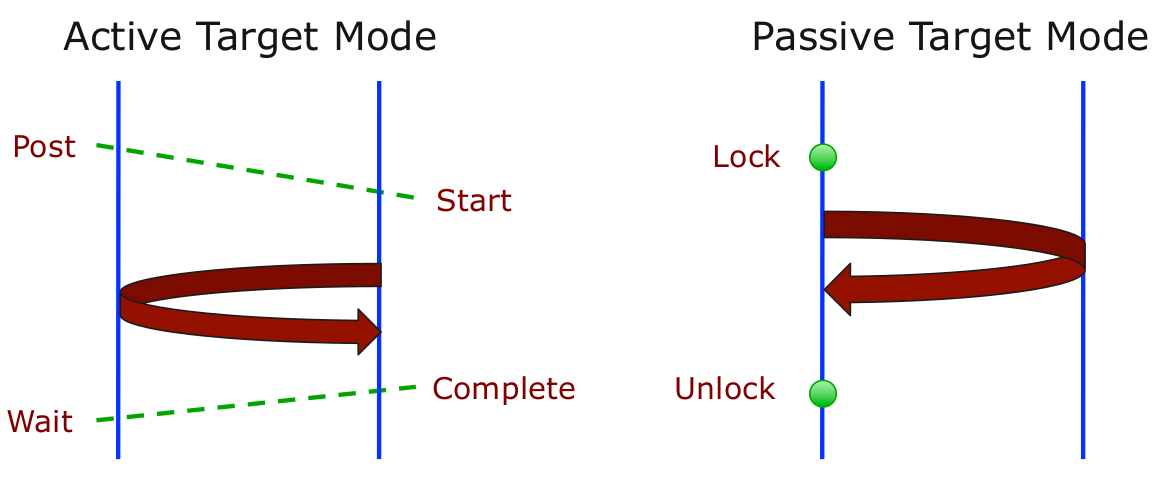
\includegraphics[width=8.0cm]{graphs/passive.png}
  \item Passive target synchronization: one-sided, asynchronous communication
  \item Target does not participate in communication operation
  \item Shared memory-like model
{\color{mycolorcode}
{\tiny
\begin{multicols}{2}
\begin{verbatim}
  int MPI_Win_lock(int lock_type, 
    int rank, int assert, MPI_Win win)

  int MPI_Win_unlock(int rank, MPI_Win win)
\end{verbatim}
\begin{verbatim}
  int MPI_Win_flush(int rank, MPI_Win win)

  int MPI_Win_flush_local(int rank, MPI_Win win)
\end{verbatim}
\end{multicols}
}
}
  \end{itemize}
\end{frame}


\begin{frame}[fragile]
  \frametitle{One-sided communication: synchronization models: passive target }
\begin{itemize}
\item Lock/Unlock: Begin/end passive mode epoch
\begin{itemize}
\item Target process does not make a corresponding MPI call
\item Can initiate multiple passive target epochs to different processes
\item Concurrent epochs to same process not allowed
\end{itemize}
\item Lock type
\begin{itemize}
\item {\color{mycolorcode}SHARED}: Other processes using shared can access concurrently
\item {\color{mycolorcode}EXCLUSIVE}: No other processes can access concurrently
\end{itemize}
\item {\color{mycolorcode}\verb|Flush|}: Remotely complete RMA operations to the target process: After completion, data can be read by target process or a different
process
\item {\color{mycolorcode}\verb|Flush_local|}: Locally complete RMA operations to the target process: after completion the user may reuse any buffers provided to put, get, or accumulate on the origin
\item Flushes can be done inside epochs
\item ``Lock'' is misleading: not a mutex, just a start and end of an epoch
\end{itemize}
\end{frame}

\subsection{Synchronization models: advanced passive target synchronization}
\begin{frame}[fragile]
  \frametitle{One-sided communication: synchronization models: advanced passive target synchronization}
{\color{mycolorcode}
\begin{verbatim}
  int MPI_Win_lock_all(int assert, MPI_Win win)
  int MPI_Win_unlock_all(MPI_Win win)
  int MPI_Win_flush_all(MPI_Win win)
  int MPI_Win_flush_local_all(int rank, MPI_Win win)
\end{verbatim}
}
  \begin{itemize}
  \item {\color{mycolorcode}\verb|Lock_all|}: Shared lock, passive target epoch to all other processes
    \begin{itemize}
      \item Expected usage is long-lived: {\color{mycolorcode}\verb|lock_all|}, {\color{mycolorcode}\verb|put/get|}, {\color{mycolorcode}\verb|flush|}, ..., {\color{mycolorcode}\verb|unlock_all|}
    \end{itemize}
    \item {\color{mycolorcode}\verb|Flush_all|} – remotely complete RMA operations to all processes
    \item {\color{mycolorcode}\verb|Flush_local_all|} - locally complete RMA operations to all processes
  \end{itemize}
\end{frame}
    
\subsection{Synchronization models: which to use?}
\begin{frame}[fragile]
  \frametitle{One-sided communication: synchronization models: which to use?}
  \begin{itemize}
  \item RMA communication has low overheads versus send/recv
    \begin{itemize}
    \item Two-sided: Matching, queuing, buffering, unexpected receives, etc...
    \item One-sided: No matching, no buffering, always ready to receive
    \item Utilize RDMA provided by high-speed interconnects (e.g.
      InfiniBand)
    \end{itemize}
  \item  Active mode: bulk synchronization
    \begin{itemize}
    \item E.g. ghost cell exchange
    \end{itemize}
  \item Passive mode: asynchronous data movement
    \begin{itemize}
    \item Useful when dataset is large, requiring memory of multiple
      nodes
    \item Also, when data access and synchronization pattern is dynamic
    \item Common use case: distributed, shared arrays
    \end{itemize}
  \item One-sided communication is still relatively new and not always well implemented in MPI, test performance
  \end{itemize}
\end{frame}

\section{Hybrid programming}
\subsection{Motivation}
\begin{frame}[fragile]
  \frametitle{Hybrid programming: motivation}
  \begin{itemize}
  \item MPI describes parallelism between processes, with separate address spaces, on the same or different physical machines
  \item Thread parallelism provides a shared-memory model within a process on one physical machine
  \item Using multithreading on a single machine is typically much faster then pure MPI since there is less overhead:
    \begin{itemize}
    \item No need to maintain buffers on sending and receiving side, no need to copy data to/from buffers
    \item Threads can share memory while each process has its own
    \end{itemize}
  \item In HPC one typically uses OpenMP for multithreading
  \item Other possible multithreading options: pthreads, C++11 threads, Intel TBB, Intel Cilk Plus,...
  \item However, multithreading can only work on a single machine and to run on a cluster one can either use pure MPI or combine MPI with some multithreading framework, typicall OpenMP - {\color{mycolordef}\textbf{hybrid programming}}
  \end{itemize}
\end{frame}

\subsection{Four levels of thread safety}
\begin{frame}[fragile]
  \frametitle{Hybrid programming: four levels of thread safety}
\begin{itemize}
\item In MPI+threads hybrid programming, there can be multiple threads executing simultaneously
\begin{itemize}
\item All threads share all MPI objects (communicators, requests)
\item The MPI implementation might need to take precautions to make sure the state of the MPI implementation is consistent
\end{itemize}
\item MPI defines four levels of thread safety - these are commitments the application makes to the MPI
\begin{itemize}
\item {\color{mycolorcode}\verb|MPI_THREAD_SINGLE|}: only one thread exists in the application
\item {\color{mycolorcode}\verb|MPI_THREAD_FUNNELED|}: multithreaded, but only the main thread makes MPI calls (the one that called {\color{mycolorcode}\verb|MPI_Init_thread|})
\item {\color{mycolorcode}\verb|MPI_THREAD_SERIALIZED|}: multithreaded, but only one thread at a time makes MPI calls
\item {\color{mycolorcode}\verb|MPI_THREAD_MULTIPLE|}: multithreaded and any thread can make MPI calls at any time
\end{itemize}
\item Instead of {\color{mycolorcode}\verb|MPI_Init|} use
{\color{mycolorcode}
\begin{verbatim}
  int MPI_Init_thread(int *argc, char ***argv, 
    int required, int *provided)
\end{verbatim}
}
\item You ask for {\color{mycolorcode}\verb|required|} level of thread safety, you get - {\color{mycolorcode}\verb|provided|}
\end{itemize}
\end{frame}

\begin{frame}[fragile]
  \frametitle{Hybrid programming: four levels of thread safety}
\begin{itemize}
\item An implementation is not required to support levels higher than {\color{mycolorcode}\verb|MPI_THREAD_SINGLE|}; that is, an implementation is not required to be thread safe
\item A fully thread-safe implementation will support {\color{mycolorcode}\verb|MPI_THREAD_MULTIPLE|}. There is much more overhead needed from the system to support it and it might be slow. 
{\color{mycolorcode}\verb|MPI_THREAD_FUNNELED|} seems to be the most optimal choice for most hybrid applications. Benchmark performance before deciding which level of thread safety to use.
\item A program that calls {\color{mycolorcode}\verb|MPI_Init|} (instead of {\color{mycolorcode}\verb|MPI_Init_thread|}) should assume that only {\color{mycolorcode}\verb|MPI_THREAD_SINGLE|} is supported
\item A threaded MPI program that does not call {\color{mycolorcode}\verb|MPI_Init_thread|} is an incorrect program (common user error) although for many MPI implementations it might actually work fine.
\end{itemize}
\end{frame}

\subsection{MPI-3 shared memory}
\begin{frame}[fragile]
  \frametitle{Hybrid programming: MPI-3 shared memory}
\begin{itemize}
\item MPI-3 one-sided communication allows different processes to allocate shared memory through MPI
\begin{itemize}
\item {\color{mycolorcode}\verb|MPI_Win_allocate_shared|}
\end{itemize}
\item Applications can do hybrid programming using MPI or load/store accesses on the shared memory window
\item Other MPI functions can be used to synchronize access to shared memory regions
\item Can be simpler to program than threads
\item One can use {\color{mycolorcode}\verb|MPI_Comm_split_type|} with {\color{mycolorcode}\verb|split_type|} equal to {\color{mycolorcode}\verb|COMM_TYPE_SHARED|} to find for the given MPI rank all the ranks on the same physical node, it is returned as a new communicator:
{\color{mycolorcode}
\begin{verbatim}
  int MPI_Comm_split_type(MPI_Comm comm, 
    int split_type, int key,
    MPI_Info info, MPI_Comm *newcomm)
\end{verbatim}
}
\item {\color{mycolorcode}\verb|key|} controls rank ordering in the new communicator.
\end{itemize}
\end{frame}


%\section{Caching}

%\section{Naming objects}

%\section{Process management}

\section{Timing}
\begin{frame}[fragile]
  \frametitle{Timing}
\begin{itemize}
\item MPI supplies its own timing routine {\color{mycolorcode}\verb|MPI_Wtime|} which gives wall clock time
\item You call it before and after an event and subtract the values:
{\color{mycolorcode}
\begin{verbatim}
  t = MPI_Wtime();
  // something happens here
  t = MPI_Wtime() - t;
\end{verbatim}
}
\item This works on a single rank
\item If you want to measure global time of a parallel application, you might need to use barriers in front of each {\color{mycolorcode}\verb|MPI_Wait|} call
\item {\color{mycolorcode}\verb|MPI_Wtick|} gives the smallest possible timer increment
\end{itemize}
\end{frame}



\section{Random practical tips}
\begin{frame}[fragile]
  \frametitle{Random practical tips}
\begin{itemize}
\item Do not ever build your program with one MPI implementation/version and run it with another! Most likely it will not work or work incorrectly.
\item If MPI is compiled with a certain compiler, it is desirable to use the same compiler for your application and all the dependencies. Typically, when you load a module it is taken care of automatically but might be accidentally 
  overwritten by subsequent module loads
\item A typical mistake: first load some MPI and then some python with mpi4py. In that case, you would be using MPI implementation supplied with mpi4py instead of MPI you intended to use. 
Always check with ``{\color{mycolorcli}which mpirun}'' what you are actually 
using
\end{itemize}
\end{frame}

\begin{frame}[fragile]
  \frametitle{Random practical tips}
\begin{itemize}
\item {\color{mycolorcli}mpirun/mpiexec} and {\color{mycolorcli}mpicc/mpiicc/mpic++/mpiicpc/mpif77/mpif90/mpifort} have different options and might even be called differently for different MPI implementations. 
\item For example, openmpi has radically different command line syntax then Intel MPI and other mpich based implementations
\item As far as command line options are concerned, Intel MPI is documented the best and is typically one of the best implementations to use, you might want to start with it
\item To debug/profile MPI/OpenMP program use Arm (former Allinea) ddt/map. Just for profiling, Intel Parallel Studio comes with VTune, Intel Advisor, 
Intel Trace Analyzer and Collector, vectorization reports options to compiler, etc. 
Score-P is another good profiling tool.
\end{itemize}
\end{frame}


\section{References}
\begin{frame}[fragile]
  \frametitle{References}
{\tiny
\begin{verbatim}
http://mpi-forum.org
http://mpi-forum.org/docs/mpi-3.1/mpi31-report.pdf
https://www.mpich.org
https://www.mpich.org/static/docs/v3.2/www3/
http://mvapich.cse.ohio-state.edu
https://software.intel.com/en-us/intel-mpi-library
https://www.open-mpi.org
http://mpitutorial.com
https://computing.llnl.gov/tutorials/mpi/
https://hpc.llnl.gov/sites/default/files/DavidCronkSlides.pdf
http://wgropp.cs.illinois.edu/courses/cs598-s16/
https://bitbucket.org/VictorEijkhout/parallel-computing-book/src

"Using MPI: Portable Parallel Programming with the Message-Passing Interface", third edition,
by William Gropp, Ewing Lusk, Anthony Skjellum

"Using Advanced MPI: Modern Features of the Message-Passing Interface", by William Gropp, Torsten Hoefler, 
Rajeev Thakur, Ewing Lusk

HDF5 page:
https://www.hdfgroup.org
\end{verbatim}
}
\end{frame}

\section{Appendix: tutorials on demand}
\begin{frame}[fragile]
  \frametitle{Tutorials on demand}
  \begin{itemize}
    \item Currently the following tutorials are available at any time:
      \begin{itemize}
        \item Introduction to Linux and RCC
        \item Introduction to Python
        \item Distributed MPI programming in C/C++/Python
        \item Multithreading programming in OpenMP
        \item Introduction to Hadoop
        \item BigData and Machine Learning with Spark and BigDL
        \item Deep Learning with Keras and TensorFlow
        \item Deep Learning with Theano
        \item Deep Learning with PyTorch
        \item Singularity Container
      \end{itemize}
    \item More are coming: Sequence Models with Deep Learning, Reinforcement learning, Deep Learning autoencoders for dimensionality
      reduction...
    \item Requests for other topics?
  \end{itemize}
\end{frame}


\end{document}
